\ifdefined\inMainDoc\else
\documentclass[12pt,a4paper]{article}
% ================================================================
%  PRÉAMBULE COMMUN - ANNALES CORRIGÉES
%  Université de Kara - FaST - Licence Fondamentale MPC
%  Design optimisé impression noir et blanc
% ================================================================

% -- ENCODAGE & LANGUE --
\usepackage[utf8]{inputenc}
\usepackage[T1]{fontenc}
\usepackage[french]{babel}
\usepackage{lmodern}
\usepackage{microtype}

% -- MISE EN PAGE --
\usepackage[a4paper, top=2.8cm, bottom=2.5cm, left=2.5cm, right=2.5cm, headheight=14pt]{geometry}
\usepackage{setspace}
\setstretch{1.2}
\usepackage{parskip}
\setlength{\parindent}{1.2em}
\setlength{\parskip}{4pt}

% -- MATHS --
\usepackage{amsmath, amssymb, mathtools, amsthm}
\usepackage{mathrsfs}
\usepackage{dsfont}
\usepackage{bm}
\usepackage{cancel}
\usepackage{textcomp}
% Définition de \oiint (intégrale de surface fermée) sans package supplémentaire
\newcommand{\oiint}{\mathop{\iint\!\!\!\!\!\!\!\bigcirc}\limits}

% -- PHYSIQUE & CHIMIE --
\usepackage{physics}
\usepackage{siunitx}
% Lorsque physics est chargé, siunitx omet \qty. On le restaure ici :
\AtBeginDocument{\RenewCommandCopy\qty\SI}
\sisetup{locale = FR, detect-all, output-decimal-marker={,}}
% Commande de substitution pour les unités posant problème avec pdflatex
% (ohm, degreeCelsius, micro, angstrom, percent utilisent des caractères non-ASCII)
\newcommand{\qtyohm}[1]{\ensuremath{\num{#1}\,\Omega}}
\newcommand{\qtydegc}[1]{\ensuremath{\num{#1}\,{}^\circ\text{C}}}
\newcommand{\qtyangstrom}[1]{\ensuremath{\num{#1}\,\text{\AA}}}
\newcommand{\qtypercent}[1]{\ensuremath{\num{#1}\,\%}}
\newcommand{\qtyum}[1]{\ensuremath{\num{#1}\,\mu\text{m}}}
\usepackage[version=4]{mhchem}

% -- GRAPHISMES --
\usepackage{graphicx}
\usepackage{float}
\usepackage{caption}
\usepackage{subcaption}
\usepackage{wrapfig}
\usepackage{tikz}
\usetikzlibrary{calc, arrows.meta, patterns, shapes.geometric}
\usepackage{pgfplots}
\pgfplotsset{compat=1.18}

% -- TABLEAUX --
\usepackage{booktabs}
\usepackage{array}
\usepackage{tabularx}
\usepackage{multirow}

% -- LISTES --
\usepackage{enumitem}
\setlist[enumerate]{topsep=3pt, itemsep=2pt, parsep=0pt}
\setlist[itemize]{topsep=3pt, itemsep=2pt, parsep=0pt, label={.}}

% -- BOÎTES (noir et blanc) --
\usepackage{mdframed}
\usepackage{tcolorbox}
\tcbuselibrary{skins, breakable, theorems}

% Boîte EXERCICE : encadré avec filet épais, fond blanc
\newmdenv[
  linewidth=1.2pt,
  linecolor=black,
  roundcorner=3pt,
  skipabove=10pt,
  skipbelow=6pt,
  innertopmargin=8pt,
  innerbottommargin=8pt,
  innerleftmargin=10pt,
  innerrightmargin=10pt,
  backgroundcolor=white,
  frametitle={\bfseries\small Exercice},
  frametitlealignment=\raggedright,
  frametitleaboveskip=4pt,
  frametitlebelowskip=4pt,
]{boiteexercice}

% Boîte CORRIGÉ : fond gris très clair + filet fin
\newmdenv[
  linewidth=0.6pt,
  linecolor=black,
  leftline=true,
  rightline=false,
  topline=false,
  bottomline=false,
  linecolor=black,
  innerleftmargin=12pt,
  innerrightmargin=8pt,
  innertopmargin=6pt,
  innerbottommargin=6pt,
  backgroundcolor=gray!8,
  skipabove=4pt,
  skipbelow=8pt,
]{boitecorrige}

% Boîte RÉSUMÉ DE COURS : double encadré
\newmdenv[
  linewidth=0.8pt,
  linecolor=black,
  roundcorner=2pt,
  backgroundcolor=gray!12,
  innertopmargin=10pt,
  innerbottommargin=10pt,
  innerleftmargin=12pt,
  innerrightmargin=12pt,
  skipabove=12pt,
  skipbelow=8pt,
]{boiteresume}

% Boîte ATTENTION/REMARQUE : barre gauche épaisse
\newmdenv[
  leftline=true,
  rightline=false,
  topline=false,
  bottomline=false,
  linewidth=3pt,
  linecolor=black,
  backgroundcolor=gray!5,
  innerleftmargin=12pt,
  innerrightmargin=8pt,
  innertopmargin=5pt,
  innerbottommargin=5pt,
  skipabove=6pt,
  skipbelow=6pt,
]{boiteremarque}

% -- DIFFICULTÉ DES EXERCICES --
\newcommand{\facile}{$\star$}
\newcommand{\moyen}{$\star\!\star$}
\newcommand{\difficile}{$\star\!\star\!\star$}
\newcommand{\niveau}[1]{\hfill\textbf{#1}\hspace{2pt}}

% -- EN-TÊTES ET PIEDS DE PAGE --
\usepackage{fancyhdr}
\pagestyle{fancy}
\fancyhf{}
\renewcommand{\headrulewidth}{0.5pt}
\renewcommand{\footrulewidth}{0.3pt}

% -- HYPERLIENS --
\usepackage[hidelinks]{hyperref}
\hypersetup{
    colorlinks=false,
    pdftitle={Annale Corrigée - Licence MPC - Université de Kara}
}

% -- TITRES --
\usepackage{titlesec}
\titleformat{\section}{\Large\bfseries}{\thesection.}{0.8em}{}[\vspace{2pt}\hrule\vspace{4pt}]
\titleformat{\subsection}{\large\bfseries}{\thesubsection.}{0.7em}{}
\titleformat{\subsubsection}{\normalsize\bfseries}{\thesubsubsection.}{0.6em}{}

% -- THÉORÈMES --
\theoremstyle{definition}
\newtheorem{defn}{Définition}[section]
\newtheorem{prop}{Propriété}[section]
\newtheorem{thm}{Théorème}[section]
\newtheorem{corol}{Corollaire}[section]
\newtheorem{exemple}{Exemple}[section]

% -- COMMANDES MATHÉMATIQUES UTILES --
\newcommand{\vect}[1]{\overrightarrow{#1}}
\newcommand{\R}{\mathbb{R}}
\newcommand{\N}{\mathbb{N}}
\newcommand{\Z}{\mathbb{Z}}
\newcommand{\C}{\mathbb{C}}
\renewcommand{\d}{\mathrm{d}}
\newcommand{\deriv}[2]{\dfrac{\d #1}{\d #2}}
\newcommand{\dpart}[2]{\dfrac{\partial #1}{\partial #2}}
\newcommand{\rot}{\overrightarrow{\mathrm{rot}}\,}
\renewcommand{\div}{\mathrm{div}\,}
\renewcommand{\grad}{\overrightarrow{\mathrm{grad}}\,}
\newcommand{\e}{\mathrm{e}}
\newcommand{\ii}{\mathrm{i}}
\renewcommand{\Tr}{\mathrm{Tr}}

% Numérotation des équations par section
\numberwithin{equation}{section}

% -- RÉSULTATS ENCADRÉS --
\newcommand{\res}[1]{\[\boxed{#1}\]}

% -- REMARQUE INLINE --
\newcommand{\rmq}[1]{\begin{boiteremarque}\textbf{Remarque.} #1\end{boiteremarque}}

% -- MISE EN VALEUR DU RÉSULTAT FINAL --
\newcommand{\reponse}[1]{%
  \begin{center}
    \fbox{\begin{minipage}{0.92\textwidth}\centering #1\end{minipage}}
  \end{center}%
}


\lhead{\small\textit{Électrostatique - Licence 1}}
\rhead{\small\textit{FaST, Université de Kara}}
\cfoot{\thepage}

\begin{document}
\fi

\begin{center}
  {\LARGE\bfseries ÉLECTROSTATIQUE ET MAGNÉTOSTATIQUE}\\[0.3cm]
  {\normalsize Licence 1 - Mathématiques, Physique et Chimie}\\[0.1cm]
  \rule{0.7\textwidth}{0.8pt}
\end{center}

\section*{Résumé du cours}

\begin{boiteresume}

\textbf{1. Loi de Coulomb.} La force exercée par une charge $q_1$ sur une charge $q_2$ placée à la distance $r$ est :
\[
\vec{F}_{1\to2} = \frac{q_1 q_2}{4\pi\varepsilon_0 r^2}\,\hat{u}_{12}
\]
avec $\varepsilon_0 \approx \qty{8.85e-12}{F.m^{-1}}$ la permittivité du vide.

\textbf{2. Champ électrique et potentiel.} Le champ créé par une charge ponctuelle $q$ en un point $M$ à distance $r$ est $\vec{E} = \frac{q}{4\pi\varepsilon_0 r^2}\hat{u}$. Le potentiel électrique : $V = \frac{q}{4\pi\varepsilon_0 r}$. Relation : $\vec{E} = -\overrightarrow{\text{grad}}\,V$.

\textbf{3. Théorème de Gauss.} Le flux du champ électrique à travers une surface fermée $S$ est proportionnel à la charge intérieure $Q_{int}$ :
\[
\oiint_S \vec{E}\cdot\d\vec{S} = \frac{Q_{int}}{\varepsilon_0}
\]

\textbf{4. Énergie électrostatique.} L'énergie potentielle d'une charge $q$ dans un potentiel $V$ est $E_p = qV$. L'énergie d'un condensateur plan : $E = \frac{Q^2}{2C} = \frac{1}{2}CV^2 = \frac{QU}{2}$.

\textbf{5. Condensateur plan.} Capacité : $C = \varepsilon_0 S/d$ (sous vide), $C = \varepsilon_r\varepsilon_0 S/d$ (avec diélectrique). Champ uniforme entre les armatures : $E = U/d$.

\textbf{6. Champ magnétostatique.} Pour une distribution de courant, le théorème d'Ampère donne :
$\oint_C \vec{B}\cdot\d\vec{l} = \mu_0 I_{\text{enlacé}}$. Pour un solénoïde infini de $n$ spires par mètre : $B = \mu_0 n I$.

\end{boiteresume}

\newpage
\section{Électrostatique}

\subsection*{Exercice 1 - Champ et potentiel d'une charge ponctuelle \niveau{\facile}}

\begin{boiteexercice}
Une charge $q = \qty{5e-9}{C}$ est placée à l'origine.
\begin{enumerate}
  \item Calculer le champ électrique $\vec{E}$ et le potentiel $V$ au point $M$ situé à $r = \qty{10}{cm}$ de $q$.
  \item Calculer la force exercée sur une charge de test $q' = \qty{-2e-9}{C}$ placée en $M$.
  \item Calculer le travail effectué par la force électrostatique pour amener $q'$ de l'infini jusqu'en $M$.
\end{enumerate}
\textbf{Donnée :} $k = 1/(4\pi\varepsilon_0) = \qty{9e9}{N.m^2.C^{-2}}$.
\end{boiteexercice}

\begin{boitecorrige}
\textbf{1.} À $r = \qty{0.1}{m}$ :
\[
E = \frac{kq}{r^2} = \frac{9\times10^9\times5\times10^{-9}}{(0{,}1)^2} = \frac{45}{0{,}01} = \qty{4500}{V.m^{-1}}
\]
\[
V = \frac{kq}{r} = \frac{9\times10^9\times5\times10^{-9}}{0{,}1} = \qty{450}{V}
\]

\textbf{2.} La force est attractive ($q$ et $q'$ de signes opposés) :
\[
F = \frac{k|q||q'|}{r^2} = \frac{9\times10^9\times5\times10^{-9}\times2\times10^{-9}}{(0{,}1)^2} = \qty{9e-6}{N}
\]
Elle est dirigée vers $q$ (vers l'origine).

\textbf{3.} Le travail pour amener $q'$ de l'infini jusqu'en $M$ est égal à l'énergie potentielle en $M$ (l'énergie à l'infini est nulle) :
\[
W = q'V(M) = (-2\times10^{-9})\times450 = \qty{-9e-7}{J}
\]

\begin{center}
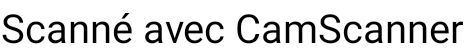
\includegraphics[width=0.7\textwidth]{images/electrostatique/elecst-007-000.png}
\captionof{figure}{\small Lignes de champ électrique $\vec{E}$ créées par une charge ponctuelle : radiales et divergentes.}
\end{center}
\end{boitecorrige}

\subsection*{Exercice 2 - Théorème de Gauss : sphère chargée uniformément \niveau{\moyen}}

\begin{boiteexercice}
Une sphère de rayon $R$ porte une charge totale $Q$ répartie uniformément en volume.
\begin{enumerate}
  \item Calculer le champ $\vec{E}$ en tout point de l'espace ($r<R$ et $r>R$).
  \item En déduire le potentiel $V(r)$ en tout point, avec $V(\infty) = 0$.
  \item Tracer qualitativement $E(r)$ et $V(r)$.
\end{enumerate}
\end{boiteexercice}

\begin{boitecorrige}
Par symétrie sphérique, $\vec{E} = E(r)\hat{r}$. On applique le théorème de Gauss sur une sphère de rayon $r$ centrée à l'origine.

\textbf{Pour $r > R$ :} $Q_{int} = Q$, donc $4\pi r^2 E = Q/\varepsilon_0$, soit :
\[
\boxed{E(r>R) = \frac{Q}{4\pi\varepsilon_0 r^2}}
\]
La sphère se comporte comme une charge ponctuelle vue de l'extérieur.

\textbf{Pour $r < R$ :} La charge intérieure est $Q_{int} = Q(r/R)^3$ (proportionnelle au volume). Donc $4\pi r^2 E = Q r^3/(R^3\varepsilon_0)$, soit :
\[
\boxed{E(r<R) = \frac{Qr}{4\pi\varepsilon_0 R^3}}
\]
Le champ est proportionnel à $r$ à l'intérieur.

\textbf{Potentiel :} En intégrant $\vec{E} = -\grad V$ avec $V(\infty)=0$ :
\begin{itemize}
  \item Pour $r>R$ : $V(r) = \dfrac{Q}{4\pi\varepsilon_0 r}$.
  \item Pour $r<R$ : $V(r) = \dfrac{Q}{4\pi\varepsilon_0}\left(\dfrac{3}{2R}-\dfrac{r^2}{2R^3}\right)$.
\end{itemize}
Le potentiel est maximum au centre : $V(0) = \dfrac{3Q}{8\pi\varepsilon_0 R} = \dfrac{3}{2}V(R)$.

\begin{center}
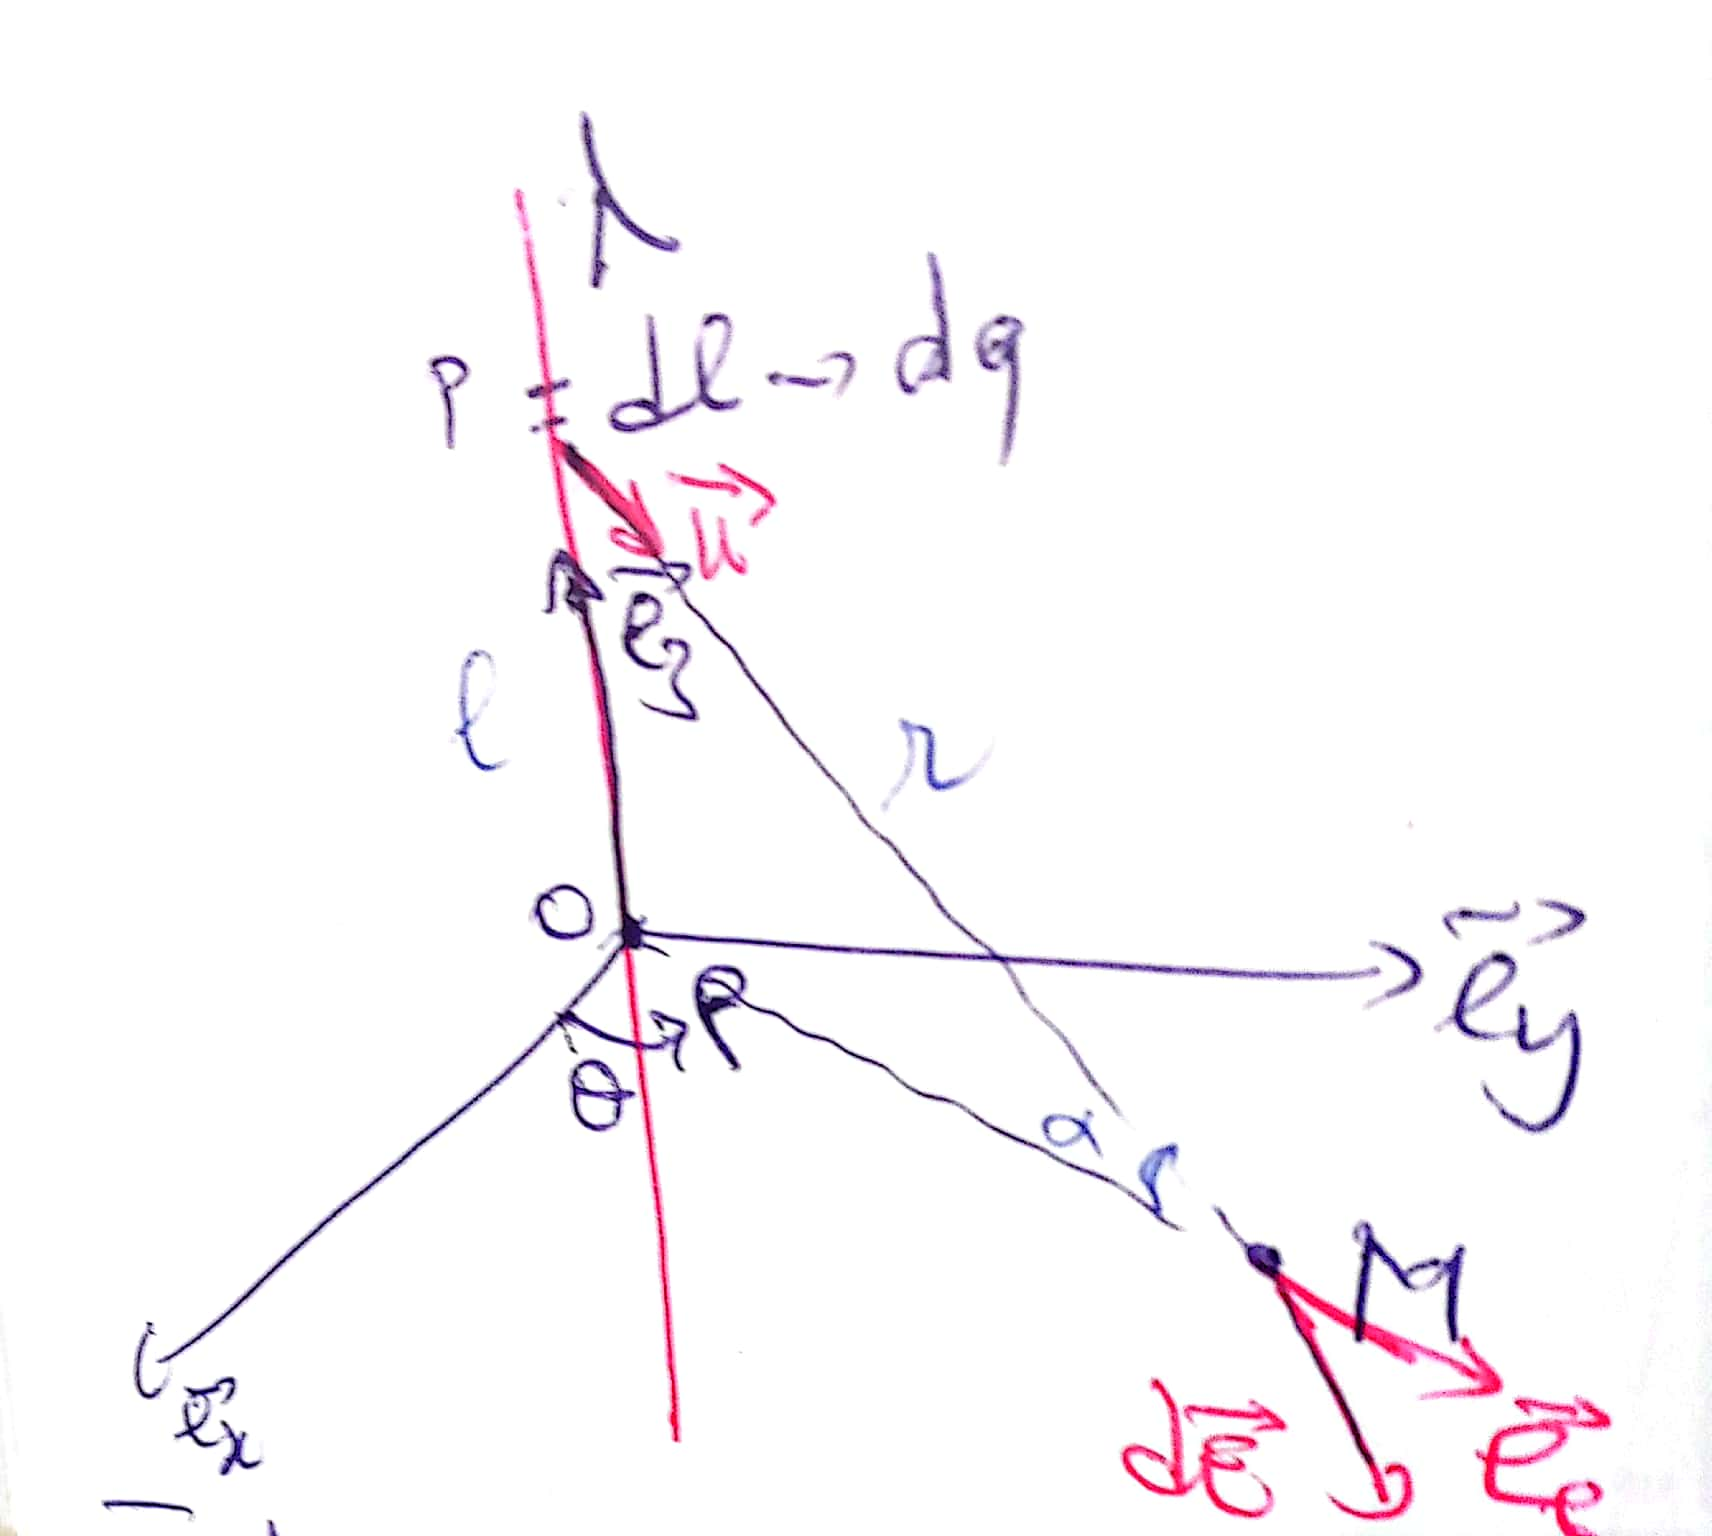
\includegraphics[width=0.7\textwidth]{images/electrostatique/elecst-007-001.png}
\captionof{figure}{\small Sphère chargée uniformément en volume : surface de Gauss sphérique et lignes de champ radial.}
\end{center}
\end{boitecorrige}

\subsection*{Exercice 3 - Condensateur plan \niveau{\facile}}

\begin{boiteexercice}
Un condensateur plan est constitué de deux armatures parallèles de surface $S = \qty{100}{cm^2}$, séparées d'une distance $d = \qty{2}{mm}$ dans le vide.
\begin{enumerate}
  \item Calculer sa capacité $C$.
  \item Il est chargé sous une tension $U = \qty{100}{V}$. Calculer la charge $Q$, le champ $E$ entre les armatures, et l'énergie stockée $W$.
  \item On insère un diélectrique de permittivité relative $\varepsilon_r = 4$ entre les armatures (à tension constante). Donner les nouvelles valeurs de $C$, $Q$ et $W$.
\end{enumerate}
\end{boiteexercice}

\begin{boitecorrige}
\textbf{1.} $C = \varepsilon_0 S/d = 8{,}85\times10^{-12}\times10^{-2}/(2\times10^{-3}) = \qty{44.25}{pF}$.

\textbf{2.} $Q = CU = 44{,}25\times10^{-12}\times100 = \qty{4.425}{nC}$.
$E = U/d = 100/(2\times10^{-3}) = \qty{50000}{V.m^{-1}}$.
$W = \frac{1}{2}CU^2 = \frac{1}{2}\times44{,}25\times10^{-12}\times10^4 = \qty{221}{pJ}$.

\textbf{3.} Avec le diélectrique (tension constante $U = \qty{100}{V}$) :
$C' = \varepsilon_r C = 4\times44{,}25 = \qty{177}{pF}$.
$Q' = C'U = \qty{17.7}{nC}$.
$W' = \frac{1}{2}C'U^2 = 4W = \qty{884}{pJ}$.

L'énergie augmente car le générateur a fourni de l'énergie supplémentaire pour maintenir la tension constante pendant l'insertion.

\begin{center}
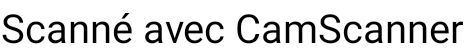
\includegraphics[width=0.7\textwidth]{images/electrostatique/elecst-009-002.png}
\captionof{figure}{\small Condensateur plan : armatures métalliques parallèles et champ $\vec{E}$ uniforme entre les plaques.}
\end{center}
\end{boitecorrige}

\subsection*{Exercice 4 - Théorème d'Ampère : solénoïde et fil infini \niveau{\moyen}}

\begin{boiteexercice}
\begin{enumerate}
  \item Un fil rectiligne infini parcouru par un courant $I = \qty{10}{A}$. Calculer le champ magnétique $B$ à la distance $r = \qty{5}{cm}$ du fil.
  \item Un solénoïde de longueur $L = \qty{20}{cm}$, comportant $N = 500$ spires, parcouru par $I = \qty{2}{A}$. Calculer le champ $B$ à l'intérieur.
  \item Calculer le flux magnétique à travers une spire de rayon $a = \qty{1}{cm}$ du solénoïde.
\end{enumerate}
\textbf{Donnée :} $\mu_0 = 4\pi\times10^{-7}\,\text{H.m}^{-1}$.
\end{boiteexercice}

\begin{boitecorrige}
\textbf{1.} Pour un fil infini, par symétrie cylindrique, le théorème d'Ampère sur un cercle de rayon $r$ donne $B\times 2\pi r = \mu_0 I$, d'où :
\[
B = \frac{\mu_0 I}{2\pi r} = \frac{4\pi\times10^{-7}\times10}{2\pi\times0{,}05} = \qty{40}{\mu T}
\]

\begin{center}
\begin{tikzpicture}[scale=1.0]
  % Fil rectiligne infini (axe z)
  \draw[very thick, gray!70] (0,-2.5) -- (0,2.5);
  \draw[->, very thick, gray!80] (0,0) -- (0,1.8) node[right, font=\small] {$I\,\hat{z}$};
  % Contour d'Ampère circulaire
  \draw[blue!70, thick, dashed] (0,0) ellipse (1.5 and 0.45);
  \draw[->, blue!70, thick] (1.5,0) arc (0:30:1.5 and 0.45);
  \node[blue!80, font=\small] at (2.2, 0) {contour d'Ampère};
  % Rayon r
  \draw[<->, red!70] (0,0) -- (1.5,0) node[midway, above, font=\small] {$r$};
  % Vecteur B tangentiel
  \draw[->, red!80, thick] (1.5, 0.3) arc (90:150:0.5);
  \node[red!80, font=\small] at (2.0, 0.55) {$\vec{B}$};
\end{tikzpicture}
\captionof{figure}{\small Symétrie cylindrique : le fil infini (gris) est le centre du contour d'Ampère circulaire (bleu) de rayon $r$. Le champ $\vec{B}$ est orthoradial.}
\end{center}

\textbf{2.} À l'intérieur d'un solénoïde de densité linéique de spires $n = N/L = 500/0{,}2 = 2500\,\text{spires.m}^{-1}$ :
\[
B = \mu_0 n I = 4\pi\times10^{-7}\times2500\times2 \approx \qty{6.28}{mT}
\]

\textbf{3.} Le flux à travers une spire de section $\pi a^2$ :
\[
\Phi = B\times\pi a^2 = 6{,}28\times10^{-3}\times\pi\times(10^{-2})^2 \approx \qty{1.97e-6}{Wb}
\]
\end{boitecorrige}


\subsection*{Exercice 5 - Distribution linéique : anneau chargé \niveau{\moyen}}

\begin{boiteexercice}
Un anneau de rayon $R = \qty{5}{cm}$ porte une charge totale $Q = \qty{2e-9}{C}$ uniformément répartie.
\begin{enumerate}
  \item Calculer le champ électrique $E$ au centre de l'anneau.
  \item Exprimer le champ électrique $E(z)$ sur l'axe de l'anneau à une distance $z$ du centre.
  \item Calculer $E(z)$ pour $z = \qty{3}{cm}$.
  \item Pour quelle valeur de $z$ le champ est-il maximal sur l'axe ?
\end{enumerate}
\textbf{Donnée :} $k = 1/(4\pi\varepsilon_0) = \qty{9e9}{N.m^2.C^{-2}}$.
\end{boiteexercice}

\begin{boitecorrige}
\textbf{1.} Par symétrie, les composantes radiales du champ se compensent en tout point de l'anneau. Au centre ($z=0$), toutes les contributions se compensent par symétrie azimutale : $\boxed{E_{centre} = 0}$.

\textbf{2.} Champ sur l'axe : chaque élément de charge $\d q$ crée un champ élémentaire. Par symétrie de révolution, seule la composante axiale $\d E_z$ survit. Pour un élément $\d q$ à distance $r = \sqrt{R^2+z^2}$ du point $P$ sur l'axe :
\[
\d E_z = \frac{k\,\d q}{R^2+z^2}\cdot\frac{z}{\sqrt{R^2+z^2}} = \frac{k\,\d q\,z}{(R^2+z^2)^{3/2}}
\]
En intégrant sur tout l'anneau :
\[
\boxed{E(z) = \frac{kQz}{(R^2+z^2)^{3/2}}}
\]

\textbf{3.} Pour $z = \qty{0.03}{m}$, $R = \qty{0.05}{m}$ :
\begin{align}
E &= \frac{9\times10^9 \times 2\times10^{-9} \times 0{,}03}{((0{,}05)^2+(0{,}03)^2)^{3/2}} \notag \\
&= \frac{0{,}54}{(0{,}0025+0{,}0009)^{3/2}} = \frac{0{,}54}{(0{,}0034)^{3/2}}
\end{align}
$(0{,}0034)^{3/2} = (0{,}0034)^1 \times (0{,}0034)^{1/2} = 0{,}0034 \times 0{,}05831 \approx 1{,}982\times10^{-4}$
\[
E \approx \frac{0{,}54}{1{,}982\times10^{-4}} \approx \qty{2724}{V.m^{-1}}
\]

\textbf{4.} On maximise $E(z)$ en dérivant et en annulant :
\[
\frac{\d E}{\d z} = kQ\frac{(R^2+z^2)^{3/2} - z\cdot\frac{3}{2}(R^2+z^2)^{1/2}\cdot2z}{(R^2+z^2)^3} = 0
\]
Le numérateur s'annule quand $(R^2+z^2) - 3z^2 = 0$, soit $R^2 = 2z^2$, donc :
\[
z_{max} = \frac{R}{\sqrt{2}} = \frac{0{,}05}{\sqrt{2}} \approx \qty{3.54}{cm}
\]

\begin{center}
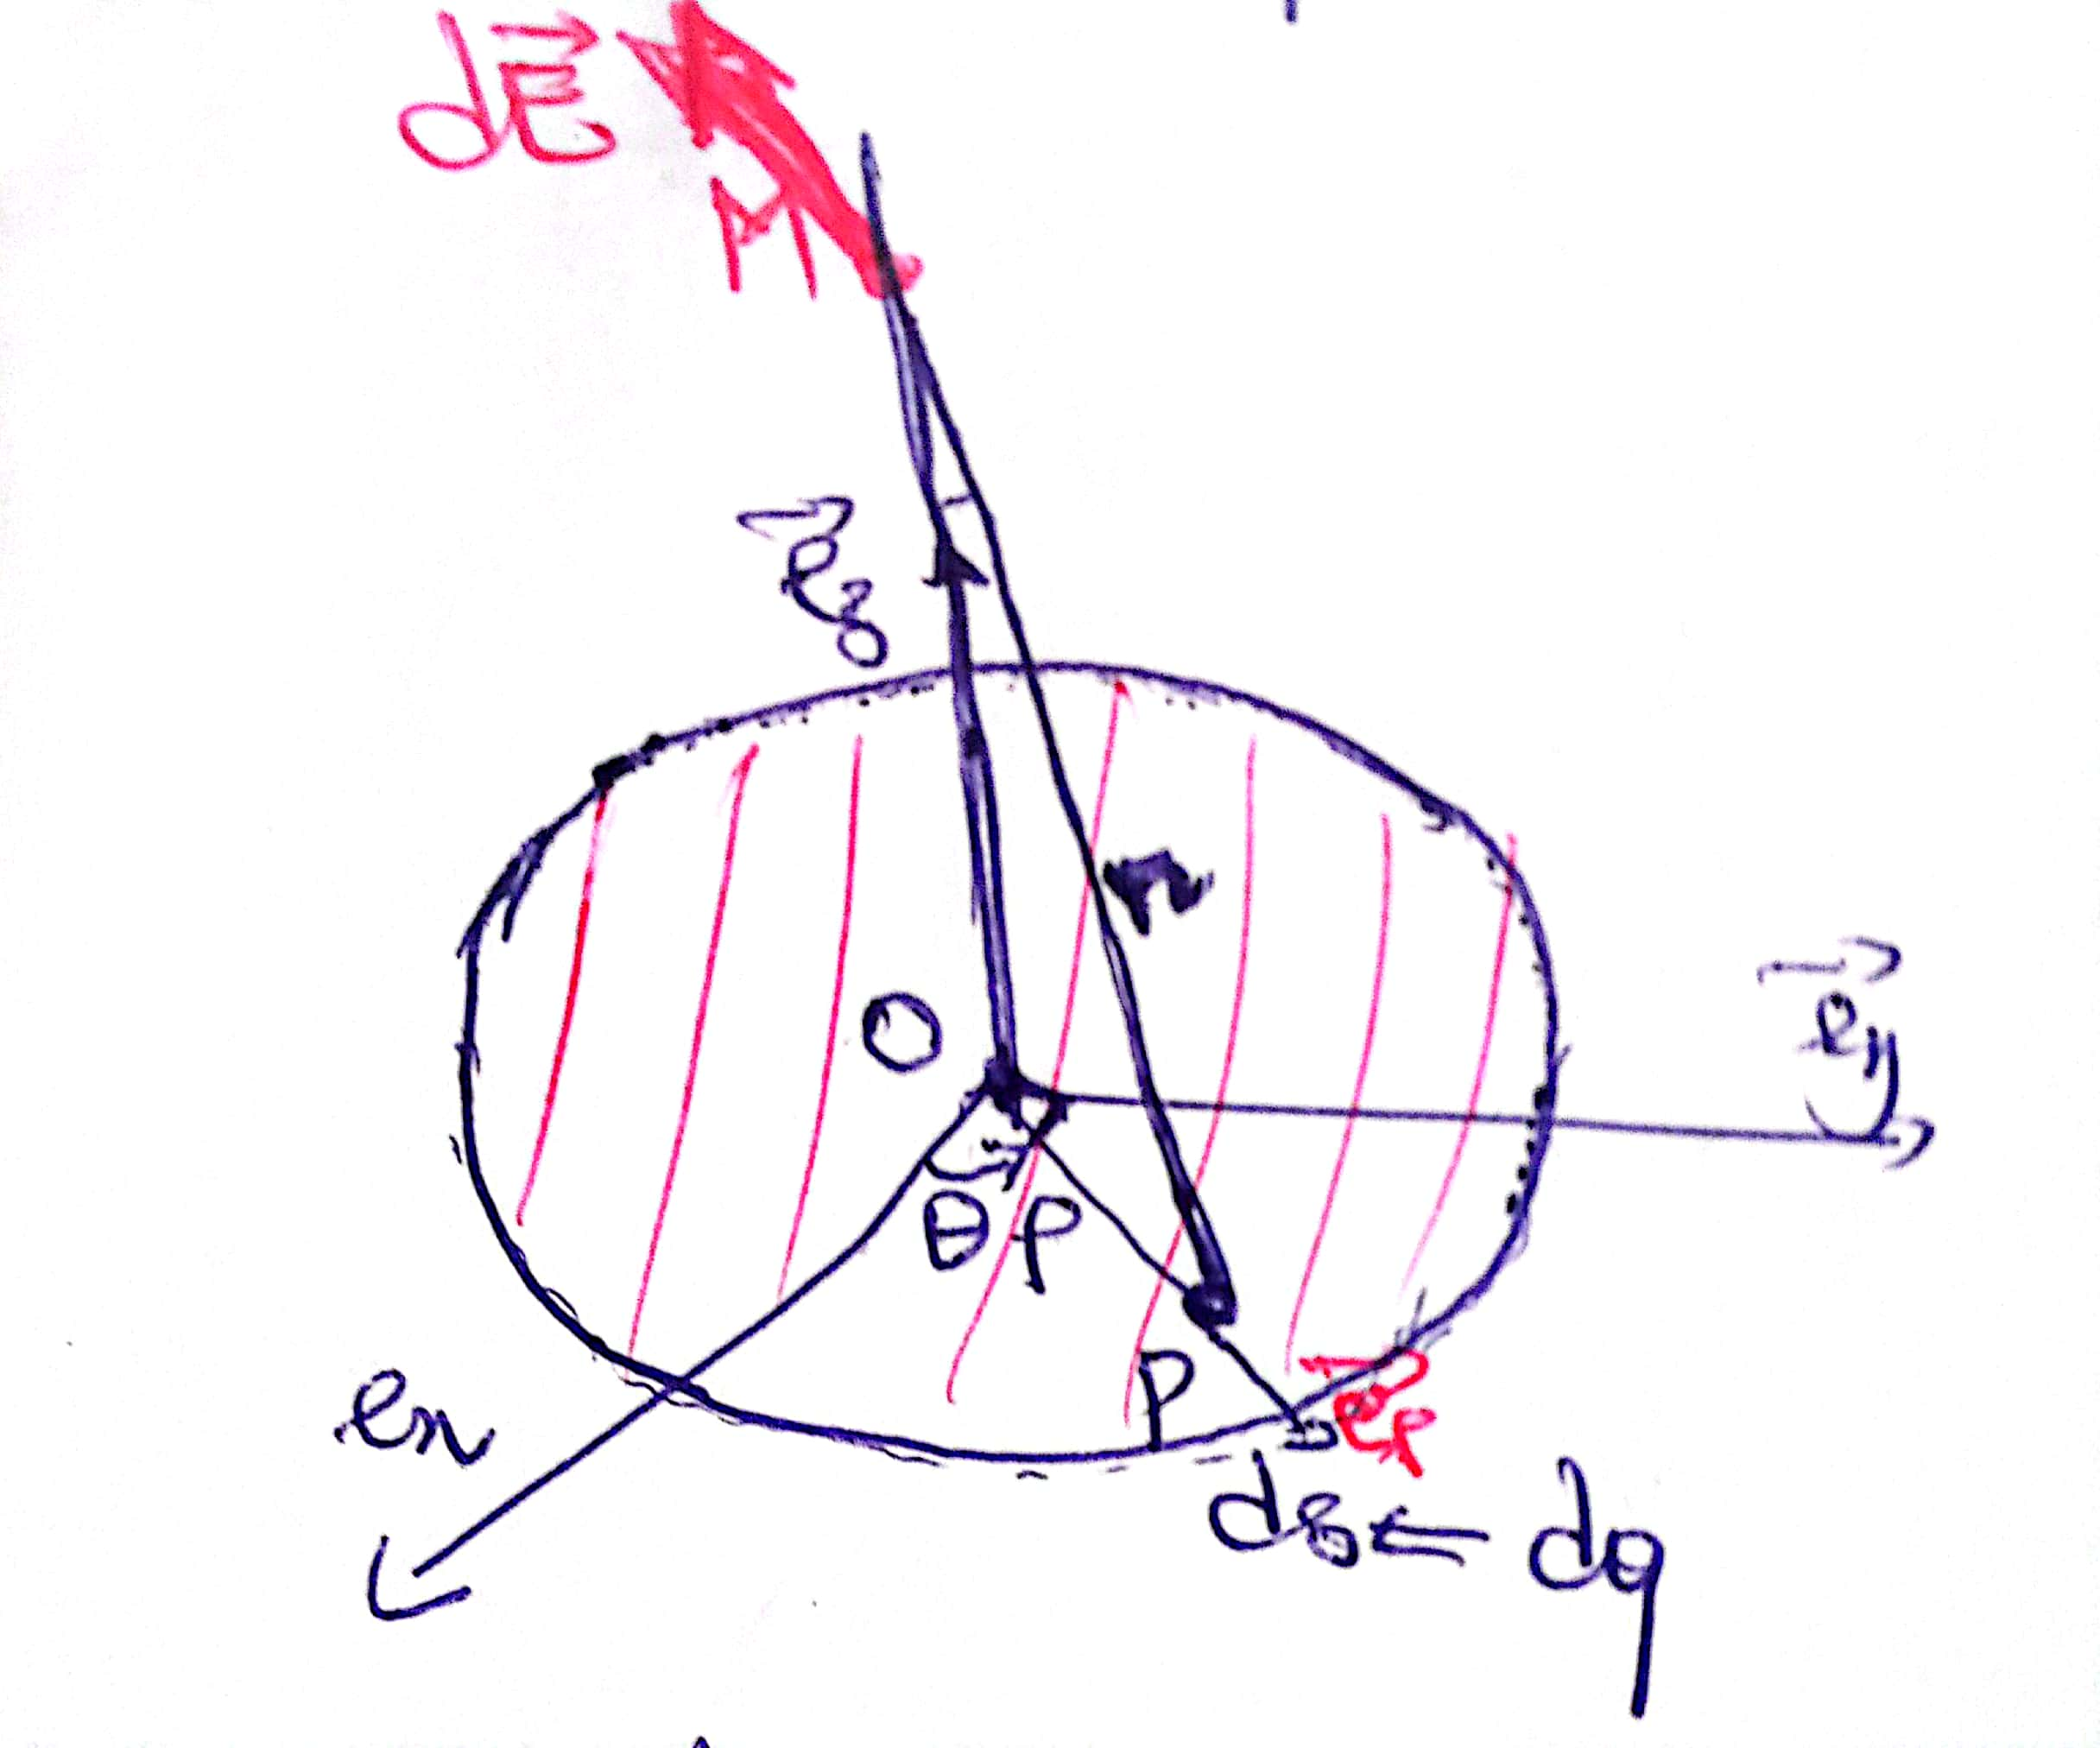
\includegraphics[width=0.7\textwidth]{images/electrostatique/elecst-009-003.png}
\captionof{figure}{\small Anneau chargé : élément $\d q$ et champ élémentaire $\d\vec{E}$ sur l'axe de révolution.}
\end{center}
\end{boitecorrige}

\subsection*{Exercice 6 - Condensateur plan chargé \niveau{\facile}}

\newpage
\begin{boiteexercice}
Un condensateur plan est formé de deux plaques parallèles de surface $S = \qty{200}{cm^2}$, distantes de $d = \qty{2}{mm}$, soumises à une tension $V = \qty{500}{V}$.
\begin{enumerate}
  \item Calculer le champ électrique $E$ entre les armatures.
  \item Calculer la capacité $C = \varepsilon_0 S/d$.
  \item Calculer la charge $Q$ sur les armatures.
  \item Calculer l'énergie stockée $U = \frac{1}{2}CV^2$.
\end{enumerate}
\textbf{Donnée :} $\varepsilon_0 = \qty{8.85e-12}{F.m^{-1}}$.
\end{boiteexercice}

\begin{boitecorrige}
\textbf{1.} Champ uniforme entre les plaques :
\[
E = \frac{V}{d} = \frac{500}{2\times10^{-3}} = \qty{2.5e5}{V.m^{-1}}
\]

\textbf{2.} Capacité :
\[
C = \frac{\varepsilon_0 S}{d} = \frac{8{,}85\times10^{-12}\times200\times10^{-4}}{2\times10^{-3}}
= 88{,}5\times10^{-12}\,\text{F} \approx \qty{88.5}{pF}
\]

\textbf{3.} Charge sur les armatures :
\[
Q = CV = 88{,}5\times10^{-12}\times500 = \qty{44.25}{nC}
\]

\textbf{4.} Énergie stockée :
\[
U = \frac{1}{2}CV^2 = \frac{1}{2}\times88{,}5\times10^{-12}\times(500)^2 = \frac{1}{2}\times88{,}5\times10^{-12}\times2{,}5\times10^5 \approx \qty{11.1}{\mu J}
\]
\end{boitecorrige}

\subsection*{Exercice 7 - Théorème de Gauss : sphère uniformément chargée \niveau{\moyen}}

\begin{boiteexercice}
Une sphère isolante de rayon $R = \qty{10}{cm}$ porte une charge totale $Q = \qty{1e-8}{C}$ répartie uniformément en volume (densité volumique $\rho = Q/(\frac{4}{3}\pi R^3)$).
\begin{enumerate}
  \item Appliquer le théorème de Gauss pour calculer $\vec{E}$ à l'intérieur ($r < R$).
  \item Calculer $\vec{E}$ à l'extérieur ($r > R$).
  \item Calculer $E$ à $r = \qty{5}{cm}$ et à $r = \qty{20}{cm}$.
\end{enumerate}
\end{boiteexercice}

\begin{boitecorrige}
Par symétrie sphérique, $\vec{E} = E(r)\,\hat{r}$.

\textbf{1. À l'intérieur ($r < R$) :} La charge enfermée dans une sphère de rayon $r$ est :
\[
Q_{int} = \rho \cdot \frac{4}{3}\pi r^3 = Q\cdot\frac{r^3}{R^3}
\]
Le théorème de Gauss donne $E(r)\cdot 4\pi r^2 = Q_{int}/\varepsilon_0$ :
\[
\boxed{E(r<R) = \frac{Qr}{4\pi\varepsilon_0 R^3}}
\]
Le champ croît linéairement avec $r$ à l'intérieur.

\textbf{2. À l'extérieur ($r > R$) :} Toute la charge $Q$ est enfermée :
\[
E(r>R)\cdot 4\pi r^2 = \frac{Q}{\varepsilon_0} \quad \Rightarrow \quad \boxed{E(r>R) = \frac{Q}{4\pi\varepsilon_0 r^2}}
\]
La sphère se comporte comme une charge ponctuelle.

\textbf{3.} Pour $r = \qty{0.05}{m}$ (intérieur) :
\[
E = \frac{9\times10^9\times10^{-8}\times0{,}05}{(0{,}10)^3} = \frac{4{,}5\times10^0}{10^{-3}} = \qty{4500}{V.m^{-1}}
\]
Pour $r = \qty{0.20}{m}$ (extérieur) :
\[
E = \frac{9\times10^9\times10^{-8}}{(0{,}20)^2} = \frac{90}{0{,}04} = \qty{2250}{V.m^{-1}}
\]
\end{boitecorrige}

\subsection*{Exercice 8 - Plan infini chargé \niveau{\moyen}}

\begin{boiteexercice}
Un plan infini porte une densité surfacique de charges $\sigma = \qty{2e-6}{C.m^{-2}}$.
\begin{enumerate}
  \item Calculer le champ électrique $E$ de part et d'autre du plan en utilisant le théorème de Gauss.
  \item Que vaut la discontinuité du champ électrique normal à la traversée du plan ?
  \item Calculer numériquement $E$.
\end{enumerate}
\end{boiteexercice}

\begin{boitecorrige}
\textbf{1.} On choisit comme surface de Gauss un cylindre de section $S$ traversant le plan, dont les deux bases sont parallèles au plan chargé. Par symétrie, le champ est perpendiculaire au plan et de même module des deux côtés.

\begin{center}
\begin{tikzpicture}[scale=0.9]
  % Plan infini chargé (en gris)
  \fill[gray!20] (-3.5,-0.12) rectangle (3.5,0.12);
  \draw[gray!60, thick] (-3.5, 0) -- (3.5, 0);
  \node[gray!80, font=\small] at (3.8, 0) {$\sigma$};
  % Cylindre de Gauss
  \draw[blue!60, thick] (-1.0,-0.12) rectangle (1.0, 0.12); % section visible
  \draw[blue!60, thick] (-1.0, 1.2) -- (-1.0,-1.2);
  \draw[blue!60, thick] (1.0, 1.2) -- (1.0,-1.2);
  \draw[blue!60, thick, dashed] (0, 1.2) ellipse (1.0 and 0.25);
  \draw[blue!60, thick] (0, -1.2) ellipse (1.0 and 0.25);
  \node[blue!70, font=\scriptsize] at (1.7, 0.8) {Surface de Gauss};
  % Flèches champ E
  \draw[->, red!70, very thick] (0, 0.12) -- (0, 1.0) node[right, font=\small] {$\vec{E}$};
  \draw[->, red!70, very thick] (0, -0.12) -- (0, -1.0) node[right, font=\small] {$\vec{E}$};
  % Section S
  \draw[<->, darkgray] (-1.0, 1.45) -- (1.0, 1.45) node[midway, above, font=\scriptsize] {$\sqrt{S}$};
\end{tikzpicture}
\captionof{figure}{\small Surface de Gauss (cylindre bleu) traversant le plan chargé $\sigma$. Le flux traverse uniquement les deux bases (surfaces parallèles au plan).}
\end{center}

Le flux total est $\Phi = 2ES$ (deux bases) et la charge enfermée est $Q_{int} = \sigma S$.

Le théorème de Gauss donne :
\[
2ES = \frac{\sigma S}{\varepsilon_0} \quad \Rightarrow \quad \boxed{E = \frac{\sigma}{2\varepsilon_0}}
\]
Le champ est dirigé vers l'extérieur du plan des deux côtés.

\textbf{2.} La discontinuité du champ normal à la traversée d'une surface chargée (surface avec $\sigma$) est :
\[
\Delta E_n = E_{au\text{-}dessus} - E_{en\text{-}dessous} = \frac{\sigma}{\varepsilon_0}
\]
Ici, $E_{au\text{-}dessus} = +\sigma/(2\varepsilon_0)$ et $E_{en\text{-}dessous} = -\sigma/(2\varepsilon_0)$, donc la saut vaut bien $\sigma/\varepsilon_0$.

\textbf{3.} Calcul numérique :
\[
E = \frac{\sigma}{2\varepsilon_0} = \frac{2\times10^{-6}}{2\times8{,}85\times10^{-12}} = \frac{2\times10^{-6}}{1{,}77\times10^{-11}} \approx \qty{1.13e5}{V.m^{-1}}
\]
\end{boitecorrige}

\subsection*{Exercice 9 - Conducteur sphérique creux \niveau{\moyen}}

\begin{boiteexercice}
Un conducteur sphérique creux a un rayon interne $R_1 = \qty{5}{cm}$ et un rayon externe $R_2 = \qty{8}{cm}$. Il porte une charge totale $Q = \qty{3e-9}{C}$.
\begin{enumerate}
  \item Décrire la distribution des charges sur le conducteur.
  \item Calculer le champ électrique dans les trois zones : $r < R_1$, $R_1 < r < R_2$ (métal), et $r > R_2$.
  \item Si l'on place une charge $q = \qty{1e-9}{C}$ à l'intérieur de la cavité, décrire à nouveau la distribution des charges.
\end{enumerate}
\end{boiteexercice}

\begin{boitecorrige}
\textbf{1. Distribution des charges (sans charge intérieure) :} Dans un conducteur à l'équilibre, le champ intérieur est nul. Toute la charge $Q$ se place sur la \textbf{surface externe} ($r = R_2$). Il n'y a aucune charge sur la surface interne ($r = R_1$) car la cavité est vide.

\textbf{2. Champ électrique :}
\begin{itemize}
  \item Zone $r < R_1$ (intérieur de la cavité) : $\vec{E} = \vec{0}$ (aucune charge enfermée).
  \item Zone $R_1 < r < R_2$ (métal) : $\vec{E} = \vec{0}$ (propriété du conducteur à l'équilibre).
  \item Zone $r > R_2$ : par Gauss, $E = \dfrac{Q}{4\pi\varepsilon_0 r^2}$.
\end{itemize}

\textbf{3. Avec charge $q$ dans la cavité :} Par le théorème de Gauss (surface dans le métal où $E=0$), la charge enfermée est nulle, donc il apparaît $-q$ sur la surface interne ($r=R_1$). La charge totale sur le conducteur étant $Q$, la surface externe porte $Q+q = \qty{3e-9}{C} + \qty{1e-9}{C} = \qty{4e-9}{C}$.

À l'extérieur ($r > R_2$) : $E = \dfrac{Q+q}{4\pi\varepsilon_0 r^2}$.

\begin{center}
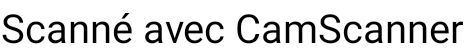
\includegraphics[width=0.7\textwidth]{images/electrostatique/elecst-013-006.png}
\captionof{figure}{\small Conducteur sphérique creux : distribution des charges sur les surfaces internes et externes.}
\end{center}
\end{boitecorrige}

\newpage
\section{Magnétostatique}

\subsection*{Exercice 10 - Champ d'un fil infini \niveau{\facile}}

\begin{boiteexercice}
Un fil rectiligne infini est parcouru par un courant $I = \qty{10}{A}$.
\begin{enumerate}
  \item En appliquant la loi de Biot-Savart (ou le théorème d'Ampère), montrer que le champ magnétique à la distance $r$ du fil est $B = \dfrac{\mu_0 I}{2\pi r}$.
  \item Calculer $B$ à $r = \qty{5}{cm}$ du fil.
  \item Calculer $B$ à $r = \qty{1}{cm}$ et $r = \qty{20}{cm}$.
\end{enumerate}
\textbf{Donnée :} $\mu_0 = 4\pi\times10^{-7}\,\text{H.m}^{-1}$.
\end{boiteexercice}

\begin{boitecorrige}
\textbf{1.} Par symétrie cylindrique, le champ $\vec{B}$ est orthoradial ($\vec{B} = B(r)\,\hat{\phi}$). On applique le théorème d'Ampère sur un cercle de rayon $r$ centré sur le fil :
\[
\oint \vec{B}\cdot\d\vec{l} = B\cdot 2\pi r = \mu_0 I_{\text{enlacé}} = \mu_0 I
\]
\[
\boxed{B = \frac{\mu_0 I}{2\pi r}}
\]

\begin{center}
\begin{tikzpicture}[scale=1.0]
  % Fil (point central avec courant sortant)
  \draw[fill=gray!40] (0,0) circle (0.18);
  \draw[thick] (-0.13,-0.13) -- (0.13,0.13);
  \draw[thick] (-0.13,0.13) -- (0.13,-0.13);
  \node[font=\small] at (0.55, 0) {$I\,(\odot)$};
  % Lignes de champ B circulaires
  \foreach \r in {0.7, 1.3, 2.0} {
    \draw[red!60, thick] (0,0) circle (\r);
    \draw[->, red!70, thick] (\r, 0) arc(0:20:\r);
  }
  % Étiquette B
  \node[red!70, font=\small] at (2.3, 0.6) {$\vec{B}$};
  % Rayon r
  \draw[<->, blue!70] (0,0) -- (1.3,0) node[midway, above, font=\small] {$r$};
  % Graphe B(r) sur le côté
  \begin{scope}[xshift=4.5cm, yshift=-1cm]
    \draw[->] (0,0) -- (3.2,0) node[right, font=\scriptsize] {$r$};
    \draw[->] (0,0) -- (0,2.5) node[above, font=\scriptsize] {$B(r)$};
    \draw[red!70, very thick, domain=0.3:3.0, samples=50]
      plot(\x, {1.2/\x});
    \node[font=\scriptsize, red!70] at (2.0, 0.9) {$B\propto 1/r$};
  \end{scope}
\end{tikzpicture}
\captionof{figure}{\small Gauche : lignes de champ $\vec{B}$ circulaires autour d'un fil infini (vue en coupe). Droite : graphe de $B(r)$ montrant la décroissance en $1/r$.}
\end{center}

\textbf{2.} À $r = \qty{0.05}{m}$ :
\[
B = \frac{4\pi\times10^{-7}\times10}{2\pi\times0{,}05} = \frac{4\times10^{-6}}{0{,}1} = \qty{40}{\mu T}
\]

\textbf{3.}
\[
B(1\,\text{cm}) = \frac{4\pi\times10^{-7}\times10}{2\pi\times0{,}01} = \qty{200}{\mu T}
\]
\[
B(20\,\text{cm}) = \frac{4\pi\times10^{-7}\times10}{2\pi\times0{,}20} = \qty{10}{\mu T}
\]
Le champ décroît en $1/r$ : en doublant la distance, $B$ est divisé par 2.
\end{boitecorrige}

\subsection*{Exercice 11 - Champ d'un solénoïde \niveau{\facile}}

\begin{boiteexercice}
Un solénoïde infini comporte $n = \qty{1000}{spires.m^{-1}}$ et est parcouru par un courant $I = \qty{2}{A}$.
\begin{enumerate}
  \item Calculer le champ magnétique $B$ à l'intérieur du solénoïde.
  \item Quel est le champ à l'extérieur du solénoïde (pour un solénoïde infini idéal) ?
  \item Calculer le flux magnétique à travers une section circulaire de rayon $a = \qty{2}{cm}$.
\end{enumerate}
\textbf{Donnée :} $\mu_0 = 4\pi\times10^{-7}\,\text{H.m}^{-1}$.
\end{boiteexercice}

\begin{boitecorrige}
\textbf{1.} On applique le théorème d'Ampère sur un rectangle de longueur $l$ dont un côté est à l'intérieur (où $B$ est uniforme et axial) et l'autre à l'extérieur (où $B\approx0$). Le courant enlacé est $I_{\text{enlacé}} = n\,l\,I$.
\[
B\cdot l = \mu_0\,n\,l\,I \quad \Rightarrow \quad \boxed{B = \mu_0 n I}
\]
\[
B = 4\pi\times10^{-7}\times1000\times2 = 4\pi\times10^{-4} \approx \qty{2.51}{mT}
\]

\textbf{2.} À l'extérieur d'un solénoïde infini idéal, le champ est nul : $B_{ext} = 0$. (En pratique, pour un solénoïde fini, il subsiste un champ résiduel faible à l'extérieur.)

\textbf{3.} Flux à travers la section $\pi a^2$ :
\[
\Phi = B\cdot\pi a^2 = 2{,}51\times10^{-3}\times\pi\times(0{,}02)^2 = 2{,}51\times10^{-3}\times1{,}257\times10^{-3} \approx \qty{3.15}{\mu Wb}
\]
\end{boitecorrige}

\subsection*{Exercice 12 - Théorème d'Ampère : tore \niveau{\difficile}}

\begin{boiteexercice}
Un tore de rayon moyen $r_0 = \qty{10}{cm}$, de section circulaire de rayon $a = \qty{1}{cm}$, comporte $N = 500$ spires portant un courant $I = \qty{3}{A}$.
\begin{enumerate}
  \item En appliquant le théorème d'Ampère $\oint \vec{B}\cdot\d\vec{l} = \mu_0 I_{\text{enlacé}}$, calculer le champ $B$ à l'intérieur du tore (à $r = r_0$).
  \item Quel est le champ à l'extérieur du tore ?
  \item Calculer l'inductance propre $L = N\Phi/I$ du tore, avec $\Phi = B\cdot\pi a^2$.
\end{enumerate}
\textbf{Donnée :} $\mu_0 = 4\pi\times10^{-7}\,\text{H.m}^{-1}$.
\end{boiteexercice}

\begin{boitecorrige}
\textbf{1.} On choisit un contour d'Ampère circulaire de rayon $r = r_0$ à l'intérieur du tore. Par symétrie de révolution, $\vec{B}$ est tangentiel et uniforme sur ce contour. Le courant enlacé est $I_{\text{enlacé}} = N\cdot I$ (toutes les spires traversent la surface délimitée par le contour) :
\[
B\cdot 2\pi r_0 = \mu_0 N I
\]
\[
B = \frac{\mu_0 N I}{2\pi r_0} = \frac{4\pi\times10^{-7}\times500\times3}{2\pi\times0{,}10} = \frac{6\pi\times10^{-4}}{\pi\times0{,}2} = \frac{6\times10^{-4}}{0{,}2} = \qty{3}{mT}
\]

\textbf{2.} Pour un contour extérieur au tore, le courant enlacé est nul (les courants aller et retour se compensent pour chaque spire) : $B_{ext} = 0$.

\textbf{3.} Inductance propre :
\[
\Phi = B\cdot\pi a^2 = 3\times10^{-3}\times\pi\times(10^{-2})^2 = 3\times10^{-3}\times\pi\times10^{-4} \approx \qty{9.42e-7}{Wb}
\]
\[
L = \frac{N\Phi}{I} = \frac{500\times9{,}42\times10^{-7}}{3} = \frac{4{,}71\times10^{-4}}{3} \approx \qty{157}{\mu H}
\]
\end{boitecorrige}


\subsection*{Exercice 13 - Anneau chargé : champ sur l'axe \niveau{\moyen}}

\begin{boiteexercice}
Un anneau de rayon $R = \qty{10}{cm}$ porte une charge totale $Q = \qty{2e-6}{C}$ répartie uniformément.
\begin{enumerate}
  \item Calculer le champ électrique en $z = 0$ (centre de l'anneau).
  \item Rappeler la formule du champ sur l'axe :
  \[
  E(z) = \frac{Qz}{4\pi\varepsilon_0(R^2+z^2)^{3/2}}
  \]
  \item Calculer numériquement $E$ en $z = R/\sqrt{2}$.
  \item Pour quelle valeur de $z$ le champ est-il maximum sur l'axe ?
\end{enumerate}
\textbf{Donnée :} $k = 1/(4\pi\varepsilon_0) = \qty{9e9}{N.m^2.C^{-2}}$.
\end{boiteexercice}

\begin{boitecorrige}
\textbf{1.} En $z = 0$, par symétrie azimutale, toutes les contributions radiales se compensent et la composante axiale de chaque élément $\d E_z = k\,\d q\cdot 0/(R^2)^{3/2} = 0$. Donc : $\boxed{E(0) = 0}$.

\textbf{2.} Chaque élément de charge $\d q$ crée sur l'axe une contribution dont seule la composante axiale $\d E_z = k\,\d q\,z/(R^2+z^2)^{3/2}$ survit par symétrie. En intégrant :
\[
E(z) = \frac{kQz}{(R^2+z^2)^{3/2}}
\]

\textbf{3.} En $z = R/\sqrt{2}$ avec $R = 0{,}1\,\text{m}$ :
\[
R^2 + z^2 = R^2 + \frac{R^2}{2} = \frac{3R^2}{2} = \frac{3\times0{,}01}{2} = 0{,}015\,\text{m}^2
\]
\[
(R^2+z^2)^{3/2} = (0{,}015)^{3/2} = 0{,}015\times\sqrt{0{,}015} = 0{,}015\times0{,}1225 \approx 1{,}837\times10^{-3}
\]
\[
E = \frac{9\times10^9\times2\times10^{-6}\times0{,}07071}{1{,}837\times10^{-3}} \approx \qty{6.93e6}{V.m^{-1}}
\]

\textbf{4.} Le maximum de $E(z)$ s'obtient en annulant $\d E/\d z = 0$. On trouve $z_{max} = R/\sqrt{2}$, soit :
\[
z_{max} = \frac{0{,}1}{\sqrt{2}} \approx \qty{7.07}{cm}
\]
\end{boitecorrige}

\subsection*{Exercice 14 - Condensateur plan : calcul complet \niveau{\facile}}

\begin{boiteexercice}
Un condensateur plan a des armatures de surface $S = \qty{0.01}{m^2}$, séparées de $d = \qty{2}{mm}$, soumises à une tension $V = \qty{500}{V}$.
\begin{enumerate}
  \item Calculer le champ électrique $E = V/d$ entre les armatures.
  \item Calculer la capacité $C = \varepsilon_0 S/d$ (dans le vide).
  \item Calculer l'énergie stockée $U = \frac{1}{2}CV^2$.
  \item Donner la densité d'énergie électrostatique $u = \frac{1}{2}\varepsilon_0 E^2$.
\end{enumerate}
\textbf{Donnée :} $\varepsilon_0 = \qty{8.85e-12}{F.m^{-1}}$.
\end{boiteexercice}

\begin{boitecorrige}
\textbf{1.} Champ uniforme entre les armatures :
\[
E = \frac{V}{d} = \frac{500}{2\times10^{-3}} = \qty{2.5e5}{V.m^{-1}}
\]

\textbf{2.} Capacité :
\[
C = \frac{\varepsilon_0 S}{d} = \frac{8{,}85\times10^{-12}\times0{,}01}{2\times10^{-3}} = \frac{8{,}85\times10^{-14}}{2\times10^{-3}} = \qty{44.25e-12}{F} \approx \qty{44.3}{pF}
\]

\textbf{3.} Énergie stockée :
\[
U = \frac{1}{2}CV^2 = \frac{1}{2}\times44{,}25\times10^{-12}\times(500)^2
\approx \qty{5.53}{\mu J}
\]

\textbf{4.} La densité volumique d'énergie électrostatique vaut :
\[
u = \frac{1}{2}\varepsilon_0 E^2 = \frac{1}{2}\times8{,}85\times10^{-12}\times(2{,}5\times10^5)^2
\approx \qty{0.276}{J.m^{-3}}
\]
Vérification : $U = u\times(S\cdot d) = 0{,}276\times(0{,}01\times2\times10^{-3}) = 0{,}276\times2\times10^{-5} \approx \qty{5.52}{\mu J}$.
\end{boitecorrige}

\subsection*{Exercice 15 - Théorème de Gauss : boule uniformément chargée \niveau{\moyen}}

\begin{boiteexercice}
Une boule isolante de rayon $R = \qty{5}{cm}$ est chargée avec une densité volumique uniforme $\rho = \qty{1e-6}{C.m^{-3}}$.
\begin{enumerate}
  \item Calculer la charge totale $Q = \rho\times\frac{4}{3}\pi R^3$.
  \item En appliquant le théorème de Gauss, exprimer $E(r)$ pour $r < R$ : $E = \rho r/(3\varepsilon_0)$.
  \item Exprimer $E(r)$ pour $r > R$ : $E = \rho R^3/(3\varepsilon_0 r^2)$.
  \item Calculer $E(R)$ par les deux formules et vérifier la continuité.
\end{enumerate}
\textbf{Donnée :} $\varepsilon_0 = \qty{8.85e-12}{F.m^{-1}}$.
\end{boiteexercice}

\begin{boitecorrige}
\textbf{1.} Charge totale :
\[
Q = \rho\times\frac{4}{3}\pi R^3 = 10^{-6}\times\frac{4\pi}{3}\times(0{,}05)^3 = 10^{-6}\times\frac{4\pi}{3}\times1{,}25\times10^{-4} \approx \qty{5.24e-10}{C}
\]

\textbf{2.} Pour $r < R$, la charge intérieure est $Q_{int} = \rho\times\frac{4}{3}\pi r^3$. Le théorème de Gauss sur une sphère de rayon $r$ :
\[
4\pi r^2 E = \frac{Q_{int}}{\varepsilon_0} = \frac{\rho\frac{4}{3}\pi r^3}{\varepsilon_0} \quad \Rightarrow \quad \boxed{E(r<R) = \frac{\rho r}{3\varepsilon_0}}
\]

\textbf{3.} Pour $r > R$, toute la charge est enfermée, $Q_{int} = Q = \rho\frac{4}{3}\pi R^3$ :
\[
4\pi r^2 E = \frac{\rho\frac{4}{3}\pi R^3}{\varepsilon_0} \quad \Rightarrow \quad \boxed{E(r>R) = \frac{\rho R^3}{3\varepsilon_0 r^2}}
\]

\textbf{4.} Calcul de $E(R)$ par les deux formules :
\[
E_{int}(R) = \frac{\rho R}{3\varepsilon_0} = \frac{10^{-6}\times0{,}05}{3\times8{,}85\times10^{-12}} = \frac{5\times10^{-8}}{2{,}655\times10^{-11}} \approx \qty{1884}{V.m^{-1}}
\]
\[
E_{ext}(R) = \frac{\rho R^3}{3\varepsilon_0 R^2} = \frac{\rho R}{3\varepsilon_0} \approx \qty{1884}{V.m^{-1}}
\]
Les deux expressions coïncident en $r = R$ : le champ est continu (pas de discontinuité car il n'y a pas de charge surfacique).

\begin{center}
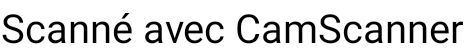
\includegraphics[width=0.7\textwidth]{images/electrostatique/elecst-012-004.png}
\captionof{figure}{\small Boule uniformément chargée : surface de Gauss sphérique et profil de champ $E(r)$.}
\end{center}
\end{boitecorrige}

\subsection*{Exercice 16 - Plan infini : champ et discontinuité \niveau{\facile}}

\begin{boiteexercice}
Un plan infini porte une densité surfacique de charges $\sigma = \qty{2e-6}{C.m^{-2}}$.
\begin{enumerate}
  \item En utilisant le théorème de Gauss avec un cylindre « pilulier », calculer $E = \sigma/(2\varepsilon_0)$ de chaque côté du plan.
  \item Calculer numériquement $E$.
  \item Exprimer la discontinuité du champ électrique normal à la traversée du plan chargé : $\Delta E_n = \sigma/\varepsilon_0$.
  \item Comparer avec un conducteur plan (surface d'un conducteur) où $E = \sigma/\varepsilon_0$.
\end{enumerate}
\textbf{Donnée :} $\varepsilon_0 = \qty{8.85e-12}{F.m^{-1}}$.
\end{boiteexercice}

\begin{boitecorrige}
\textbf{1.} Surface de Gauss : cylindre de section $S$ traversant le plan, axe perpendiculaire. Les deux bases contribuent au flux ($2ES$), le flux latéral est nul (champ parallèle aux faces latérales) :
\[
2ES = \frac{\sigma S}{\varepsilon_0} \quad \Rightarrow \quad \boxed{E = \frac{\sigma}{2\varepsilon_0}}
\]
Le champ est uniforme, perpendiculaire au plan, dirigé vers l'extérieur des deux côtés.

\textbf{2.} Application numérique :
\[
E = \frac{2\times10^{-6}}{2\times8{,}85\times10^{-12}} = \frac{2\times10^{-6}}{1{,}77\times10^{-11}} \approx \qty{1.13e5}{V.m^{-1}}
\]

\textbf{3.} Le champ est $+\sigma/(2\varepsilon_0)$ d'un côté et $-\sigma/(2\varepsilon_0)$ de l'autre (en convention vectorielle). La discontinuité de la composante normale est :
\[
\Delta E_n = E_{+} - E_{-} = \frac{\sigma}{2\varepsilon_0} - \left(-\frac{\sigma}{2\varepsilon_0}\right) = \frac{\sigma}{\varepsilon_0}
\]

\textbf{4.} Pour la surface d'un conducteur, le champ intérieur est nul. La discontinuité est $E_{ext} - 0 = \sigma/\varepsilon_0$, donc $E_{ext} = \sigma/\varepsilon_0$. C'est le double du champ d'un plan isolant, car pour le conducteur le plan est unilatéral (champ nul d'un côté).

\begin{center}
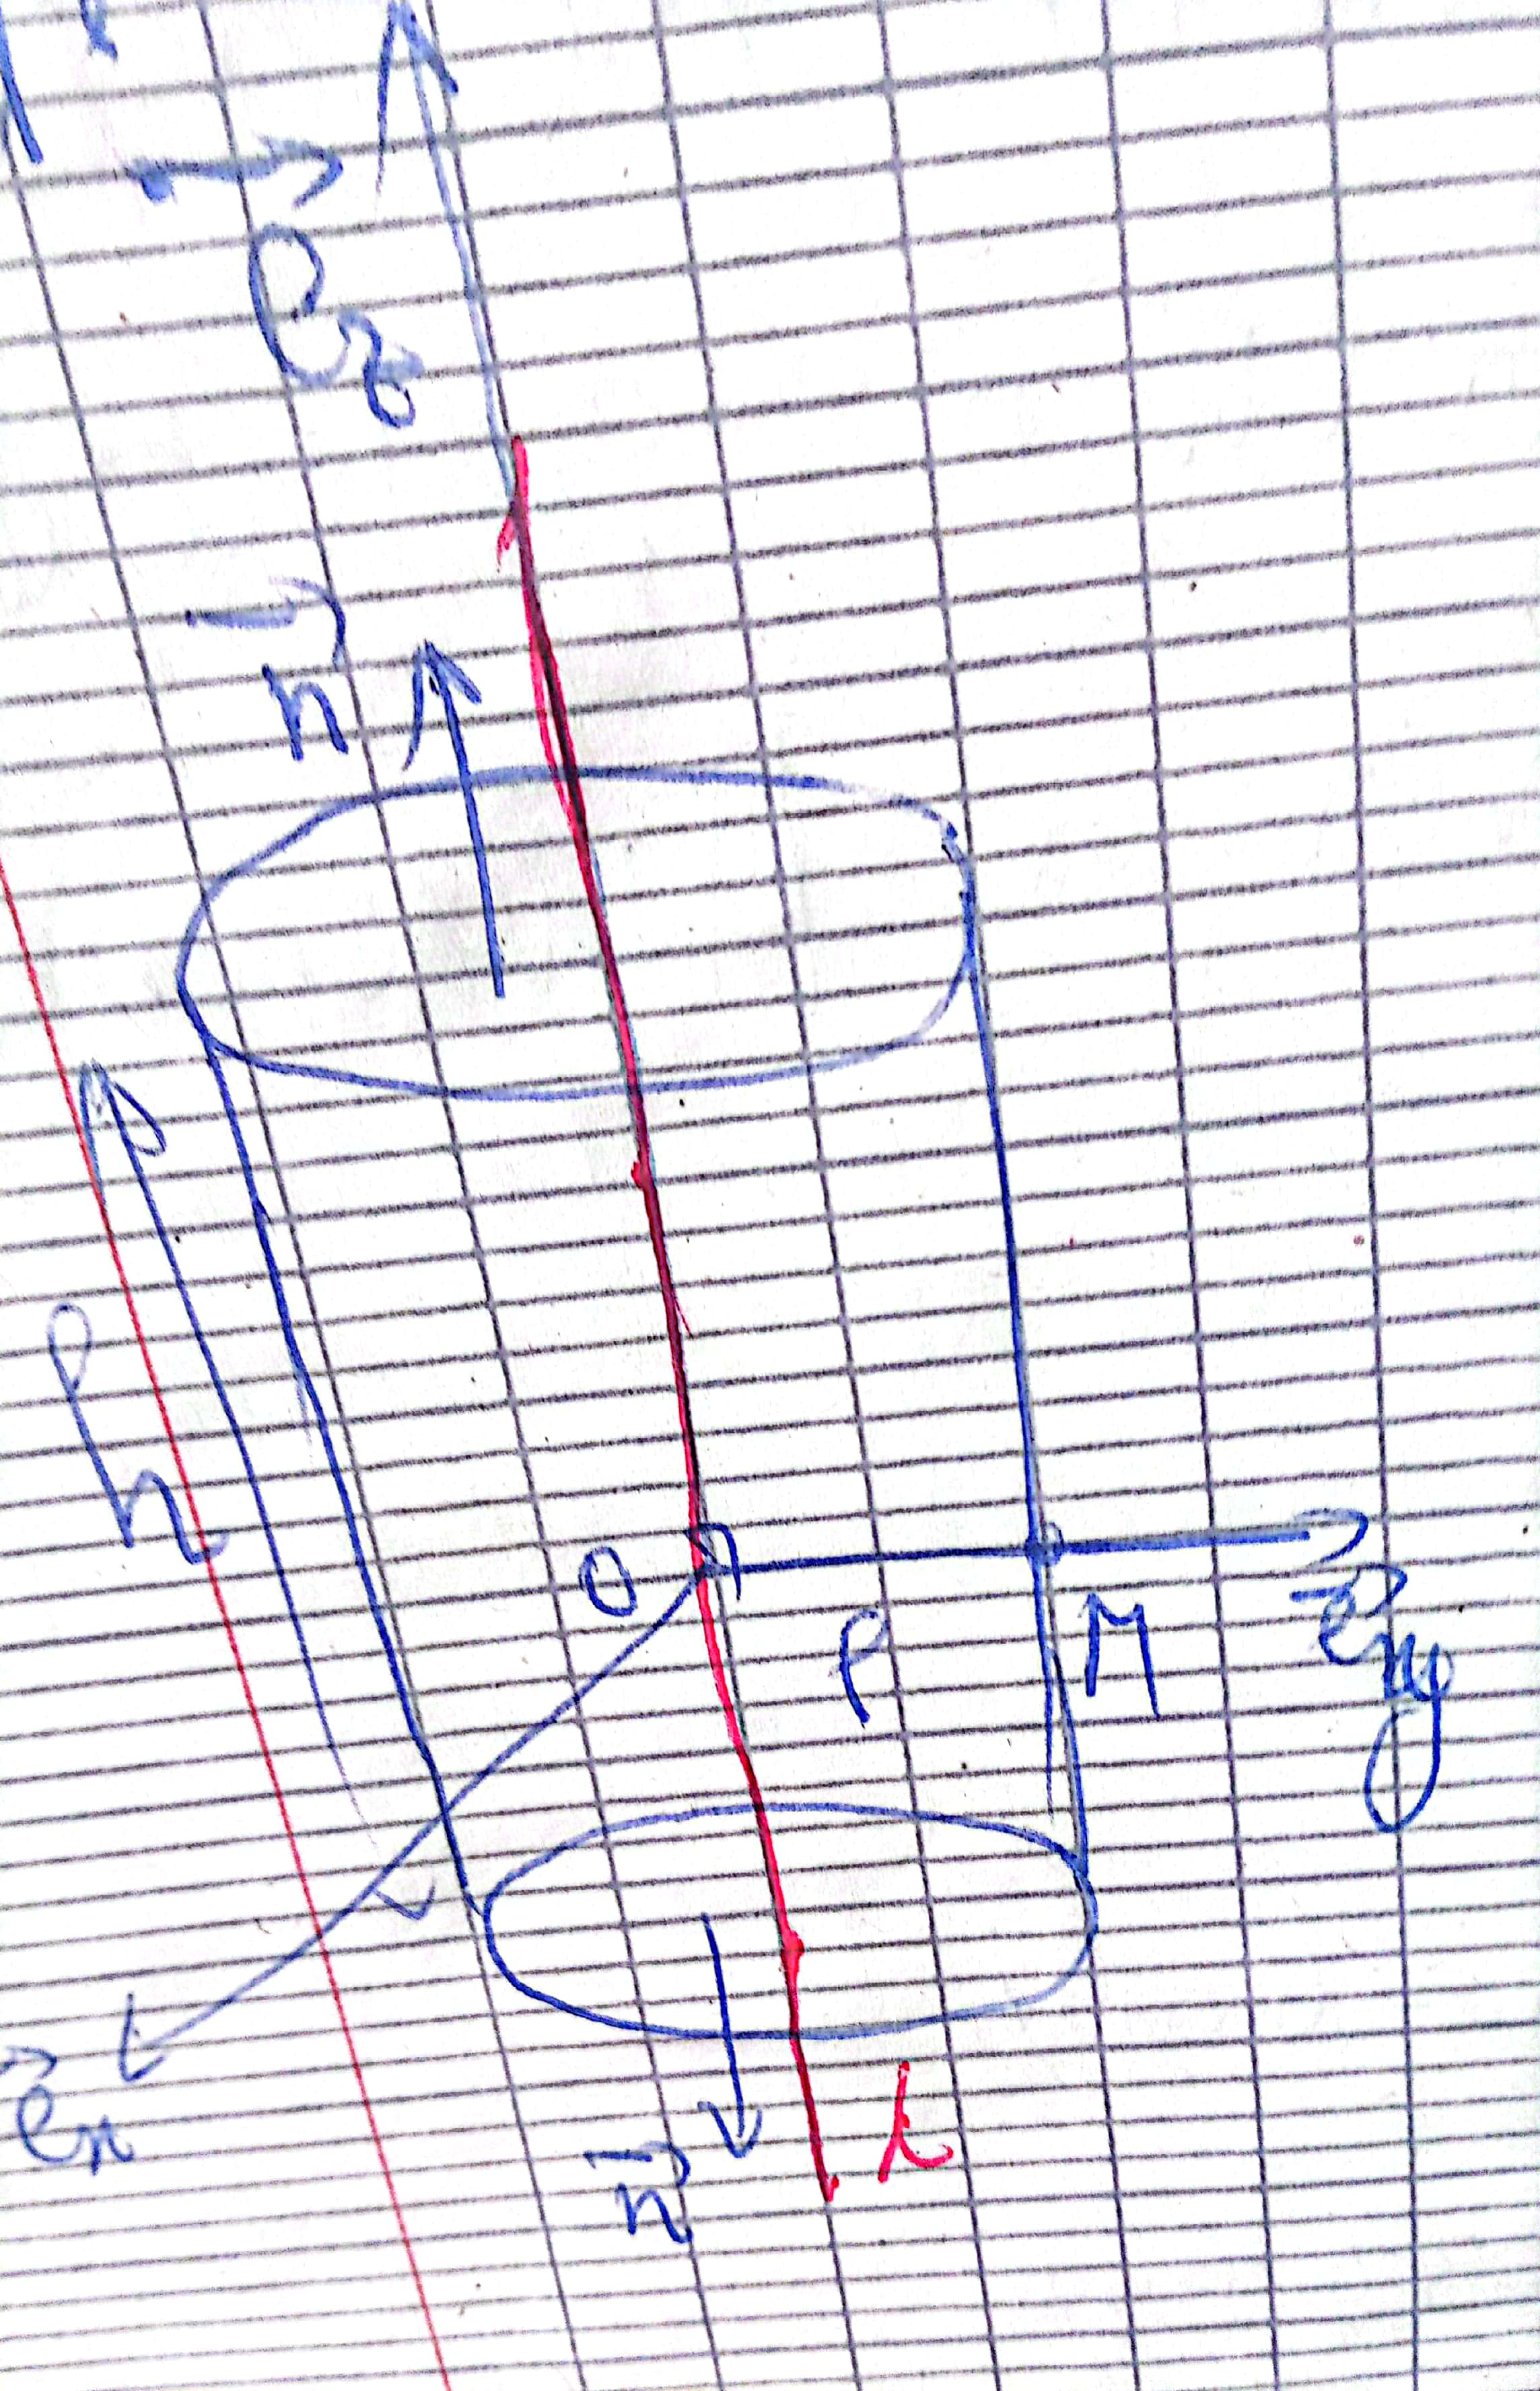
\includegraphics[width=0.7\textwidth]{images/electrostatique/elecst-012-005.png}
\captionof{figure}{\small Plan infini chargé : cylindre de Gauss « pilulier » traversant le plan, champ $\vec{E}$ perpendiculaire au plan.}
\end{center}
\end{boitecorrige}

\subsection*{Exercice 17 - Fil infini et force magnétique \niveau{\moyen}}

\begin{boiteexercice}
Un fil rectiligne infini est parcouru par un courant $I = \qty{10}{A}$.
\begin{enumerate}
  \item Calculer le champ magnétique $B$ à la distance $r = \qty{5}{cm}$ : $B = \mu_0 I/(2\pi r)$.
  \item Un second fil parallèle, de longueur $L = \qty{20}{cm}$, parcouru par $I' = \qty{5}{A}$, est placé à la même distance $r = \qty{5}{cm}$ du premier. Calculer la force exercée sur ce second fil.
  \item Les deux fils sont-ils attirés ou repoussés lorsque les courants sont dans le même sens ? dans le sens opposé ?
\end{enumerate}
\textbf{Donnée :} $\mu_0 = 4\pi\times10^{-7}\,\text{H.m}^{-1}$.
\end{boiteexercice}

\begin{boitecorrige}
\textbf{1.} Par le théorème d'Ampère (contour circulaire de rayon $r$) :
\[
B = \frac{\mu_0 I}{2\pi r} = \frac{4\pi\times10^{-7}\times10}{2\pi\times0{,}05} = \frac{4\times10^{-6}}{0{,}1} = \qty{4e-5}{T} = \qty{40}{\mu T}
\]

\textbf{2.} La force par unité de longueur sur un fil de courant $I'$ dans un champ $B$ est $F/L = I'B$. Pour la longueur $L = \qty{0.2}{m}$ :
\[
F = I' B L = 5\times4\times10^{-5}\times0{,}2 = \qty{4e-5}{N}
\]

\textbf{3.}
\begin{itemize}
  \item Courants de \textbf{même sens} : les deux fils s'attirent (force attractive). C'est la base de la définition historique de l'ampère.
  \item Courants de \textbf{sens opposés} : les deux fils se repoussent.
\end{itemize}
\end{boitecorrige}

\subsection*{Exercice 18 - Solénoïde : champ et flux \niveau{\facile}}

\begin{boiteexercice}
Un solénoïde de densité linéique $n = \qty{2000}{spires.m^{-1}}$, de rayon $R = \qty{2}{cm}$, est parcouru par un courant $I = \qty{3}{A}$.
\begin{enumerate}
  \item Calculer le champ magnétique $B = \mu_0 n I$ à l'intérieur du solénoïde.
  \item Calculer le flux magnétique à travers une section transversale : $\Phi = B\cdot\pi R^2$.
  \item Si la longueur du solénoïde est $\ell = \qty{30}{cm}$, donner le nombre total de spires $N = n\ell$ et l'inductance propre $L = N\Phi/I = \mu_0 n^2 \pi R^2 \ell$.
\end{enumerate}
\textbf{Donnée :} $\mu_0 = 4\pi\times10^{-7}\,\text{H.m}^{-1}$.
\end{boiteexercice}

\begin{boitecorrige}
\textbf{1.} Champ à l'intérieur d'un solénoïde infini :
\[
B = \mu_0 n I = 4\pi\times10^{-7}\times2000\times3 = 4\pi\times10^{-7}\times6000 = 24\pi\times10^{-4} \approx \qty{7.54}{mT}
\]

\textbf{2.} Flux à travers une section de rayon $R = \qty{0.02}{m}$ :
\[
\Phi = B\cdot\pi R^2 = 7{,}54\times10^{-3}\times\pi\times(0{,}02)^2 = 7{,}54\times10^{-3}\times\pi\times4\times10^{-4}
\]
\[
\Phi = 7{,}54\times10^{-3}\times1{,}257\times10^{-3} \approx \qty{9.47e-6}{Wb}
\]

\textbf{3.} Nombre de spires : $N = n\ell = 2000\times0{,}3 = 600\,\text{spires}$.

Inductance propre :
\[
L = \frac{N\Phi}{I} = \frac{600\times9{,}47\times10^{-6}}{3} = \frac{5{,}682\times10^{-3}}{3} \approx \qty{1.89}{mH}
\]
Vérification par la formule directe : $L = \mu_0 n^2\pi R^2\ell = 4\pi\times10^{-7}\times(2000)^2\times\pi\times(0{,}02)^2\times0{,}3 \approx \qty{1.89}{mH}$.
\end{boitecorrige}


\subsection*{Exercice 19 - Dipôle électrique : champ et potentiel \niveau{\difficile}}

\begin{boiteexercice}
Un dipôle électrique est formé de deux charges $+q$ et $-q$ séparées d'une distance $d$. On définit le moment dipolaire $\vec{p} = q\vec{d}$, dirigé de $-q$ vers $+q$, de module $p = qd$.

On travaille en coordonnées sphériques $(r, \theta)$ où $\theta$ est l'angle entre $\vec{r}$ et l'axe du dipôle, et on suppose $r \gg d$ (approximation dipolaire).

\begin{enumerate}
  \item Le potentiel électrostatique créé par le dipôle à grande distance est :
  \[
  V(r,\theta) = \frac{p\cos\theta}{4\pi\varepsilon_0\,r^2}
  \]
  Vérifier la cohérence dimensionnelle de cette expression.

  \item Les composantes du champ électrique $\vec{E} = -\overrightarrow{\text{grad}}\,V$ en coordonnées sphériques sont :
  \[
  E_r = -\frac{\partial V}{\partial r} = \frac{2p\cos\theta}{4\pi\varepsilon_0\,r^3}, \qquad
  E_\theta = -\frac{1}{r}\frac{\partial V}{\partial\theta} = \frac{p\sin\theta}{4\pi\varepsilon_0\,r^3}
  \]
  Calculer $E_r$ et $E_\theta$ à partir de $V$.

  \item Application numérique : pour une molécule d'eau ($p = \qty{6.2e-30}{C.m}$), calculer $V$ et $|\vec{E}|$ à $r = \qty{1}{nm}$ selon $\theta = 0^\circ $ et $\theta = 90^\circ $.

  \item Un dipôle $\vec{p}$ est placé dans un champ électrique extérieur uniforme $\vec{E}_0$. L'énergie potentielle d'interaction est $U = -\vec{p}\cdot\vec{E}_0$. Calculer $U$ pour $p = \qty{6.2e-30}{C.m}$ et $E_0 = \qty{1e6}{V.m^{-1}}$ pour $\theta = 0^\circ $ (dipôle aligné avec le champ) et $\theta = 90^\circ $ (dipôle perpendiculaire).

  \item Quelle est la position d'équilibre stable du dipôle dans le champ ? Justifier.
\end{enumerate}

\textbf{Données :} $\varepsilon_0 = \qty{8.85e-12}{F.m^{-1}}$, $k = 1/(4\pi\varepsilon_0) = \qty{9e9}{N.m^2.C^{-2}}$.
\end{boiteexercice}

\begin{boitecorrige}
\textbf{1. Vérification dimensionnelle.}

$[p] = \text{C}\cdot\text{m}$, $[4\pi\varepsilon_0] = \text{F.m}^{-1}\cdot\text{m} = \text{C}^2/(\text{J}\cdot\text{m}) \cdot\text{m} = \text{C}^2/\text{J}$.

\[
[V] = \frac{[\text{C}\cdot\text{m}]}{[\text{C}^2/\text{J}]\cdot[\text{m}^2]} = \frac{\text{C}\cdot\text{m}\cdot\text{J}}{\text{C}^2\cdot\text{m}^2} = \frac{\text{J}}{\text{C}\cdot\text{m}} = \frac{\text{V}}{\text{m}} \times\text{m} = \ldots
\]

On vérifie plus directement : $[p\cos\theta/(4\pi\varepsilon_0 r^2)] = \frac{\text{C}\cdot\text{m}}{\text{F.m}^{-1}\cdot\text{m}^2\cdot\text{m}} = \frac{\text{C}}{\text{F}} = \frac{\text{C}}{\text{C/V}} = \text{V}$.

\textbf{2. Calcul du champ.}

\textit{Composante radiale :}
\[
E_r = -\frac{\partial V}{\partial r} = -\frac{\partial}{\partial r}\left(\frac{p\cos\theta}{4\pi\varepsilon_0\,r^2}\right) = -p\cos\theta\cdot\frac{-2}{4\pi\varepsilon_0\,r^3} = \frac{2p\cos\theta}{4\pi\varepsilon_0\,r^3}
\]

\textit{Composante angulaire :}
\[
E_\theta = -\frac{1}{r}\frac{\partial V}{\partial\theta} = -\frac{1}{r}\cdot\frac{p}{4\pi\varepsilon_0\,r^2}\cdot(-\sin\theta) = \frac{p\sin\theta}{4\pi\varepsilon_0\,r^3}
\]

Le module du champ est :
\[
|\vec{E}| = \sqrt{E_r^2 + E_\theta^2} = \frac{p}{4\pi\varepsilon_0\,r^3}\sqrt{4\cos^2\theta + \sin^2\theta} = \frac{p}{4\pi\varepsilon_0\,r^3}\sqrt{1 + 3\cos^2\theta}
\]

\textbf{3. Application numérique} ($p = \qty{6.2e-30}{C.m}$, $r = \qty{1}{nm} = \qty{1e-9}{m}$, $k = \qty{9e9}{N.m^2.C^{-2}}$).

\textit{Selon $\theta = 0^\circ $ (axe du dipôle) :}
\[
V = \frac{kp\cos 0^\circ }{r^2} = \frac{9\times10^9\times6{,}2\times10^{-30}}{(10^{-9})^2} = \frac{5{,}58\times10^{-20}}{10^{-18}} \approx \qty{0.0558}{V}
\]
\[
|\vec{E}| = \frac{kp\sqrt{1+3}}{r^3} = \frac{9\times10^9\times6{,}2\times10^{-30}\times2}{10^{-27}} = \frac{1{,}116\times10^{-19}}{10^{-27}} \approx \qty{1.116e8}{V.m^{-1}}
\]

\textit{Selon $\theta = 90^\circ $ (plan équatorial) :}
\[
V = \frac{kp\cos 90^\circ }{r^2} = 0
\]
\[
|\vec{E}| = \frac{kp\sqrt{0+1}}{r^3} = \frac{9\times10^9\times6{,}2\times10^{-30}}{10^{-27}} = \qty{5.58e7}{V.m^{-1}}
\]
Le champ dans le plan équatorial est deux fois plus faible que sur l'axe.

\textbf{4. Énergie d'interaction.}

$U = -\vec{p}\cdot\vec{E}_0 = -pE_0\cos\theta$.

\begin{itemize}[nosep]
  \item $\theta = 0^\circ $ : $U = -pE_0 = -6{,}2\times10^{-30}\times10^6 = \qty{-6.2e-24}{J}$ (état de basse énergie).
  \item $\theta = 90^\circ $ : $U = 0$ (dipôle perpendiculaire, état d'énergie nulle).
\end{itemize}

\textbf{5. Position d'équilibre stable.}

L'équilibre stable correspond au minimum d'énergie potentielle $U = -pE_0\cos\theta$, soit $\cos\theta = +1$, c'est-à-dire $\theta = 0^\circ $ : le dipôle est aligné avec le champ ($\vec{p}$ parallèle à $\vec{E}_0$). C'est intuitivement cohérent : le champ tend à aligner les dipôles dans sa direction (c'est le phénomène de polarisation des diélectriques). À $\theta = 180^\circ $ ($\vec{p}$ antiparallèle à $\vec{E}_0$), l'énergie est maximale : c'est un équilibre instable.

\begin{center}
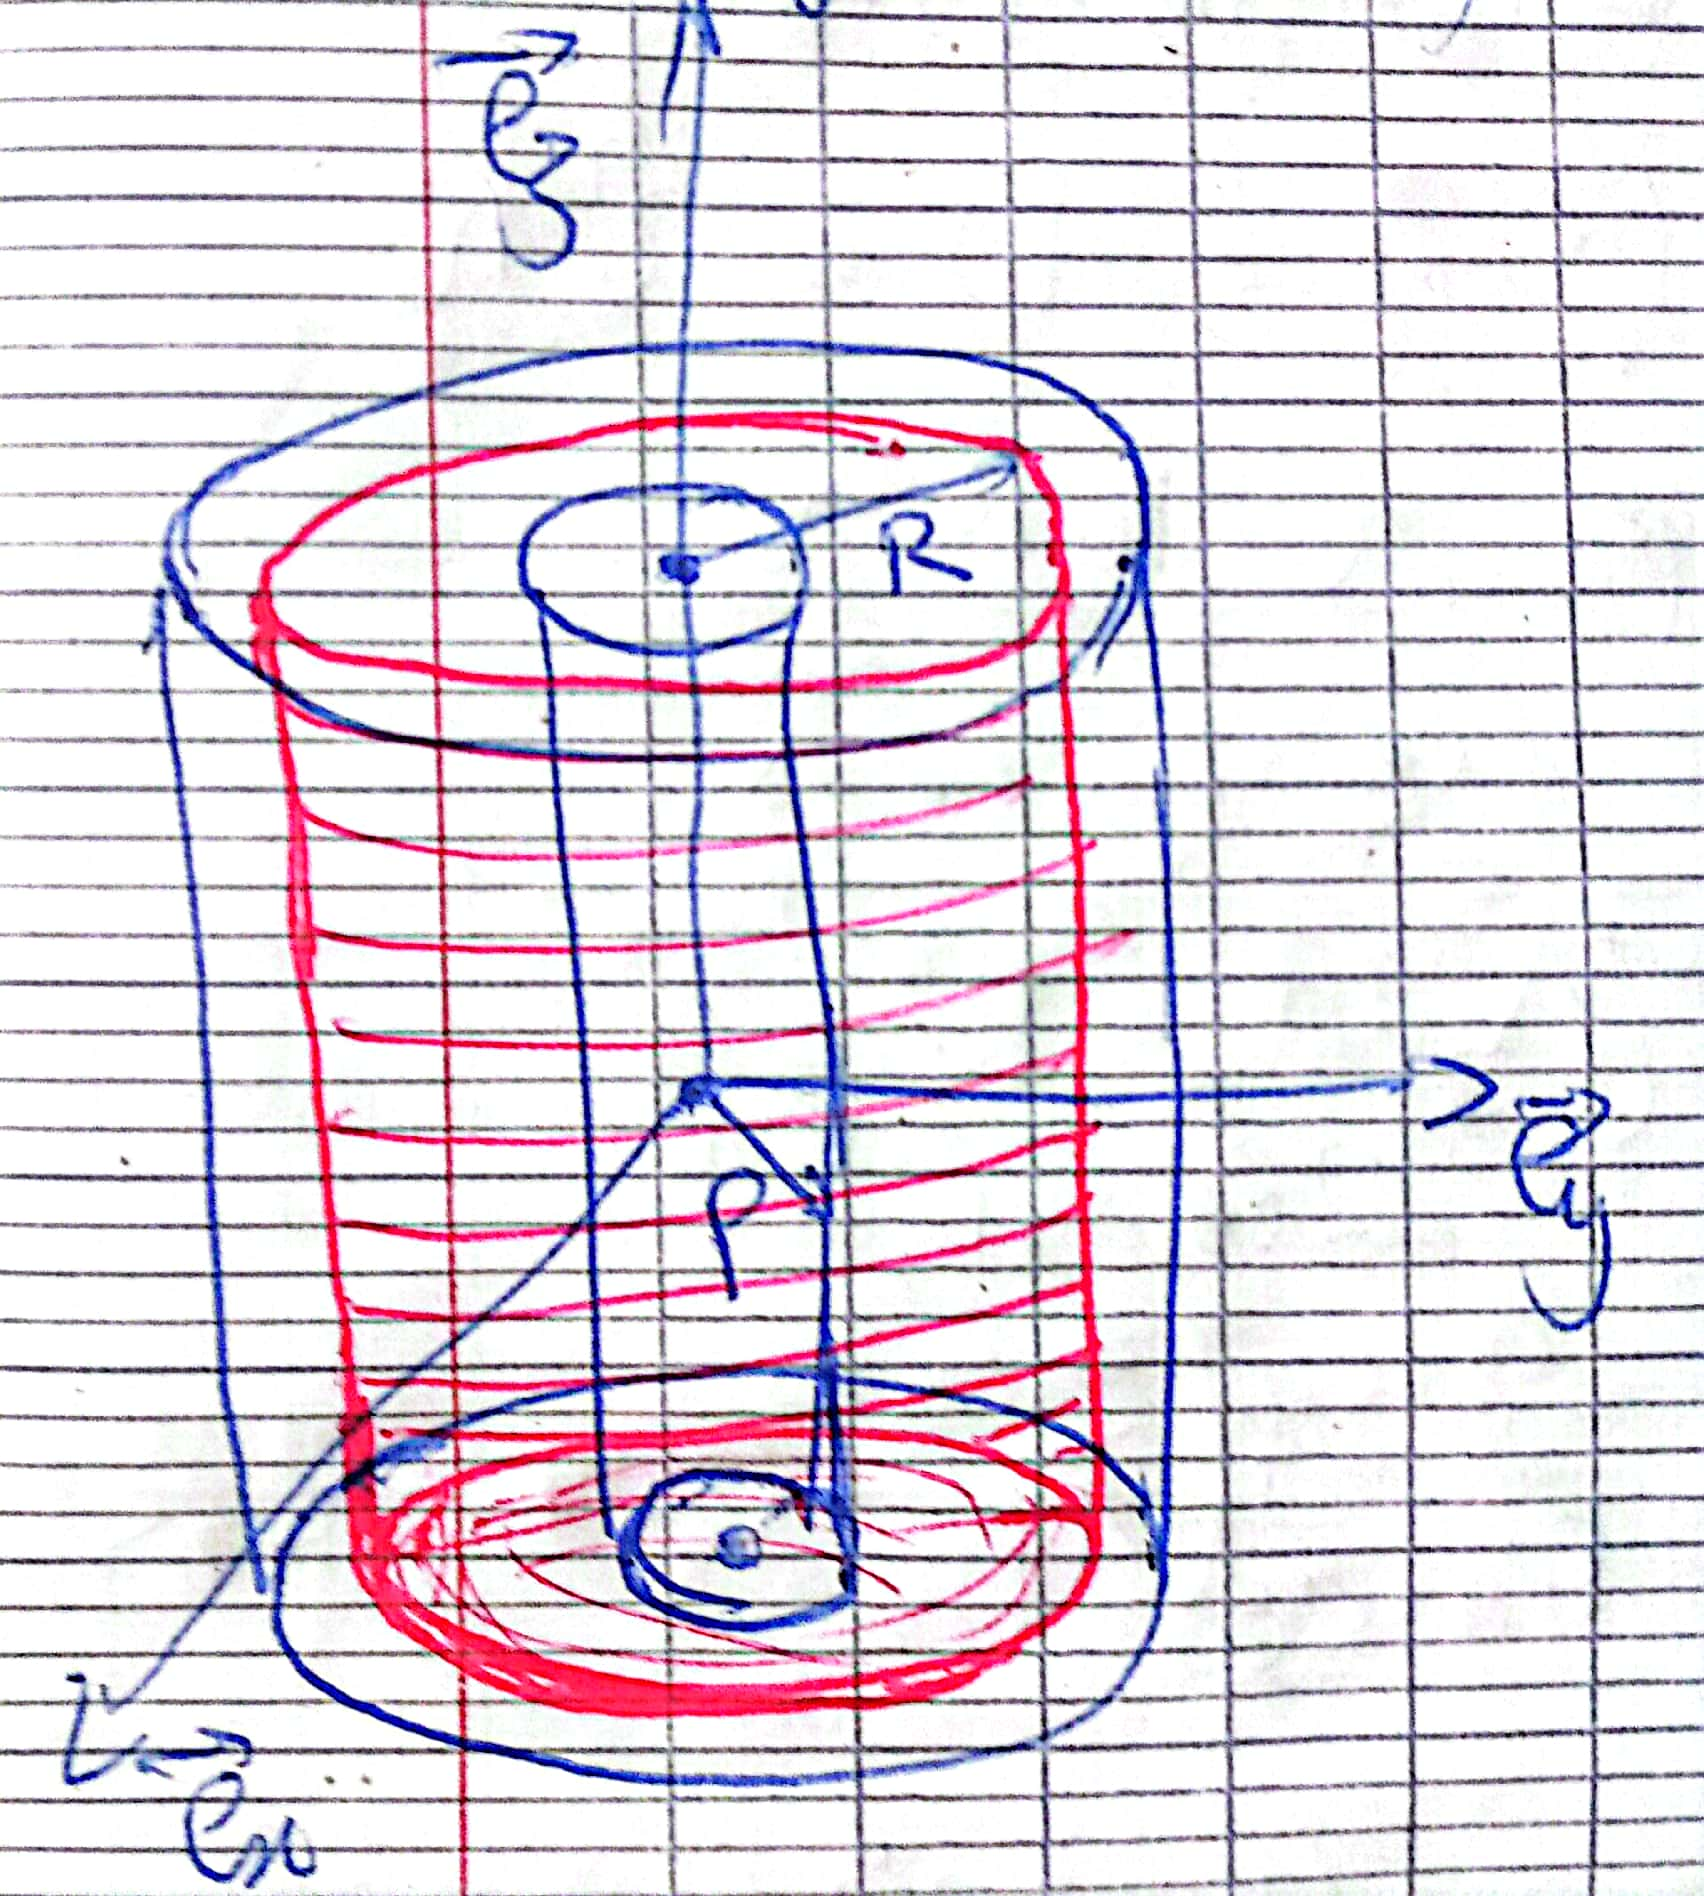
\includegraphics[width=0.7\textwidth]{images/electrostatique/elecst-013-007.png}
\captionof{figure}{\small Dipôle électrique : lignes de champ émanant de $+q$ et convergeant vers $-q$, moment dipolaire $\vec{p}$.}
\end{center}
\end{boitecorrige}

\subsection*{Exercice 20 - Énergie électrostatique d'une sphère chargée \niveau{\difficile}}

\begin{boiteexercice}
On considère une sphère conductrice de rayon $R$ portant une charge totale $Q$ répartie uniformément en surface.

\begin{enumerate}
  \item Rappeler le champ électrique $\vec{E}$ à l'intérieur ($r < R$) et à l'extérieur ($r > R$) de la sphère.
  \item L'énergie électrostatique stockée dans le champ peut se calculer par :
  \[
  U_E = \frac{\varepsilon_0}{2}\int_{\text{tout l'espace}} E^2\,\d^3r
  \]
  En intégrant sur tout l'espace, montrer que :
  \[
  U_E = \frac{Q^2}{8\pi\varepsilon_0 R}
  \]
  \item Application numérique pour une sphère de $R = \qty{10}{cm}$ portant $Q = \qty{1}{\mu C}$.
  \item À quelle tension équivalente de condensateur sphérique $C = 4\pi\varepsilon_0 R$ correspond cette énergie ($U_E = Q^2/(2C)$) ?
\end{enumerate}
\end{boiteexercice}

\begin{boitecorrige}
\textbf{1. Champ électrique.}

Pour une sphère conductrice, les charges se répartissent en surface. Par le théorème de Gauss :
\[
E(r < R) = 0 \quad \text{(intérieur d'un conducteur)}
\]
\[
E(r > R) = \frac{Q}{4\pi\varepsilon_0\,r^2} \quad \text{(identique à une charge ponctuelle)}
\]

\textbf{2. Calcul de l'énergie.}

Comme $E = 0$ à l'intérieur, seule la région extérieure ($r > R$) contribue. En coordonnées sphériques, $\d^3r = 4\pi r^2\,\d r$ :
\[
U_E = \frac{\varepsilon_0}{2}\int_R^{+\infty} E^2(r)\cdot 4\pi r^2\,\d r = \frac{\varepsilon_0}{2}\int_R^{+\infty} \left(\frac{Q}{4\pi\varepsilon_0\,r^2}\right)^2 4\pi r^2\,\d r
\]
\[
= \frac{\varepsilon_0}{2}\cdot\frac{Q^2}{16\pi^2\varepsilon_0^2}\cdot 4\pi\int_R^{+\infty} \frac{1}{r^4}\cdot r^2\,\d r = \frac{Q^2}{8\pi\varepsilon_0}\int_R^{+\infty} r^{-2}\,\d r
\]
\[
= \frac{Q^2}{8\pi\varepsilon_0}\left[\frac{-1}{r}\right]_R^{+\infty} = \frac{Q^2}{8\pi\varepsilon_0}\cdot\frac{1}{R}
\]
\[
\boxed{U_E = \frac{Q^2}{8\pi\varepsilon_0 R}}
\]

\textbf{3. Application numérique.}

\[
U_E = \frac{Q^2}{8\pi\varepsilon_0 R} = k\frac{Q^2}{2R} = \frac{9\times10^9\times(10^{-6})^2}{2\times0{,}1} = \frac{9\times10^9\times10^{-12}}{0{,}2} = \qty{45}{mJ}
\]

\textbf{4. Capacité et tension.}

La capacité d'une sphère isolée : $C = 4\pi\varepsilon_0 R = \dfrac{R}{k} = \dfrac{0{,}1}{9\times10^9} \approx \qty{11.1}{pF}$.

La relation $U_E = Q^2/(2C)$ donne :
\[
U_E = \frac{(10^{-6})^2}{2\times11{,}1\times10^{-12}} = \frac{10^{-12}}{22{,}2\times10^{-12}} \approx \qty{45}{mJ}
\]

La tension correspondante est :
\[
V = \frac{Q}{C} = \frac{kQ}{R} = \frac{9\times10^9\times10^{-6}}{0{,}1} = \qty{90000}{V} = \qty{90}{kV}
\]
Une sphère de $10\,\text{cm}$ de rayon portant $1\,\mu\text{C}$ est portée à $90\,\text{kV}$ --- cela illustre pourquoi des charges macroscopiques sur de petits objets produisent des tensions très élevées.
\end{boitecorrige}

\ifdefined\inMainDoc\else\end{document}\fi
